\PassOptionsToPackage{unicode=true}{hyperref} % options for packages loaded elsewhere
\PassOptionsToPackage{hyphens}{url}
%
\documentclass[12pt,turkish,a4paperpaper,]{report}
\usepackage{lmodern}
\usepackage{amssymb,amsmath}
\usepackage{ifxetex,ifluatex}
\usepackage{fixltx2e} % provides \textsubscript
\ifnum 0\ifxetex 1\fi\ifluatex 1\fi=0 % if pdftex
  \usepackage[T1]{fontenc}
  \usepackage[utf8]{inputenc}
  \usepackage{textcomp} % provides euro and other symbols
\else % if luatex or xelatex
  \usepackage{unicode-math}
  \defaultfontfeatures{Ligatures=TeX,Scale=MatchLowercase}
\fi
% use upquote if available, for straight quotes in verbatim environments
\IfFileExists{upquote.sty}{\usepackage{upquote}}{}
% use microtype if available
\IfFileExists{microtype.sty}{%
\usepackage[]{microtype}
\UseMicrotypeSet[protrusion]{basicmath} % disable protrusion for tt fonts
}{}
\IfFileExists{parskip.sty}{%
\usepackage{parskip}
}{% else
\setlength{\parindent}{0pt}
\setlength{\parskip}{6pt plus 2pt minus 1pt}
}
\usepackage{hyperref}
\hypersetup{
            pdfborder={0 0 0},
            breaklinks=true}
\urlstyle{same}  % don't use monospace font for urls
\usepackage{longtable,booktabs}
% Fix footnotes in tables (requires footnote package)
\IfFileExists{footnote.sty}{\usepackage{footnote}\makesavenoteenv{longtable}}{}
\usepackage{graphicx,grffile}
\makeatletter
\def\maxwidth{\ifdim\Gin@nat@width>\linewidth\linewidth\else\Gin@nat@width\fi}
\def\maxheight{\ifdim\Gin@nat@height>\textheight\textheight\else\Gin@nat@height\fi}
\makeatother
% Scale images if necessary, so that they will not overflow the page
% margins by default, and it is still possible to overwrite the defaults
% using explicit options in \includegraphics[width, height, ...]{}
\setkeys{Gin}{width=\maxwidth,height=\maxheight,keepaspectratio}
\setlength{\emergencystretch}{3em}  % prevent overfull lines
\providecommand{\tightlist}{%
  \setlength{\itemsep}{0pt}\setlength{\parskip}{0pt}}
\setcounter{secnumdepth}{5}
% Redefines (sub)paragraphs to behave more like sections
\ifx\paragraph\undefined\else
\let\oldparagraph\paragraph
\renewcommand{\paragraph}[1]{\oldparagraph{#1}\mbox{}}
\fi
\ifx\subparagraph\undefined\else
\let\oldsubparagraph\subparagraph
\renewcommand{\subparagraph}[1]{\oldsubparagraph{#1}\mbox{}}
\fi

% set default figure placement to htbp
\makeatletter
\def\fps@figure{htbp}
\makeatother


% Dizin Ayarları

% \def\contentsname{\empty}
% \setcounter{tocdepth}{6}
\usepackage[dotinlabels]{titletoc}
% \contentsmargin{2em}
\titlecontents{chapter}[0em]{\singlespace}{\makebox[4em][l]{\thecontentslabel.\quad\enspace}}{}{\titlerule*[0.75pc]{.}\contentspage}

% Sections
\dottedcontents{section}[4pc]{\singlespace}{4pc}{0.75pc}% %
\dottedcontents{subsection}[4pc]{\singlespace}{4pc}{0.75pc}% %
\dottedcontents{subsubsection}[4em]{\singlespace}{4em}{0.75pc}% %

% Dizinlere Sayfa No yazısı eklemek için
\addtocontents{toc}{~\hfill\textbf{\underline{Sayfa No}}\par}
\addtocontents{lof}{~\hfill\textbf{\underline{Sayfa No}}\par}
\addtocontents{lot}{~\hfill\textbf{\underline{Sayfa No}}\par}

% Dizin başlıklarını düzeltmek için
\setlength{\cftbeforetoctitleskip}{-8mm}
\renewcommand{\contentsname}{\hfill\normalfont\normalsize\textbf{İÇİNDEKİLER}\hfill}
\renewcommand{\cftaftertoctitle}{\hfill}
\setlength{\cftaftertoctitleskip}{28pt}

\setlength{\cftbeforeloftitleskip}{-8mm}
\renewcommand{\listfigurename}{\hfill\normalfont\normalsize\textbf{ŞEKİLLER DİZİNİ}\hfill}
\setlength{\cftafterloftitleskip}{28pt}

\setlength{\cftbeforelottitleskip}{-8mm}
\renewcommand{\listtablename}{\hfill\normalfont\normalsize\textbf{TABLOLAR DİZİNİ}\hfill}
\setlength{\cftafterlottitleskip}{28pt}

% SAYFA NUMARALARI
\usepackage{fancyhdr}
\fancypagestyle{main}{              % Başlıklar
    \fancyhf{}
    \fancyhead[C]{\thepage}
    \setlength{\headheight}{15pt}
    \renewcommand{\headrulewidth}{0.0pt}
    \pagenumbering{arabic}
    \setcounter{page}{1}
}
\pagestyle{plain}{                  % Ön Sayfalar
    \pagenumbering{Roman}
}


% Following package is used to add background image to front page
\usepackage{wallpaper}

% Table package
\usepackage{ctable}% http://ctan.org/pkg/ctable

% Deal with 'LaTeX Error: Too many unprocessed floats.'
\usepackage{morefloats}
% or use \extrafloats{100}
% add some \clearpage

% % Chapter header
% \usepackage{titlesec, blindtext, color}
% \definecolor{gray75}{gray}{0.75}
% \newcommand{\hsp}{\hspace{20pt}}
% \titleformat{\chapter}[hang]{\Huge\bfseries}{\thechapter\hsp\textcolor{gray75}{|}\hsp}{0pt}{\Huge\bfseries}

% Fonts and typesetting
\setmainfont[Scale=1.0]{Times New Roman}
\setsansfont[Scale=1.0]{Verdana}

% FONTS
\usepackage{xunicode}
\usepackage{xltxtra}
\defaultfontfeatures{Mapping=tex-text} % converts LaTeX specials (``quotes'' --- dashes etc.) to unicode
% \setromanfont[Scale=1.01,Ligatures={Common},Numbers={OldStyle}]{Palatino}
% \setromanfont[Scale=1.01,Ligatures={Common},Numbers={OldStyle}]{Adobe Caslon Pro}
%Following line controls size of code chunks
% \setmonofont[Scale=0.9]{Monaco}
%Following line controls size of figure legends
% \setsansfont[Scale=1.2]{Optima Regular}

% CODE BLOCKS
% \usepackage[utf8]{inputenc}
\usepackage{listings}
\usepackage{color}

% JAVA CODE BLOCKS
\definecolor{backcolour}{RGB}{242,242,242}
\definecolor{javared}{rgb}{0.6,0,0}
\definecolor{javagreen}{rgb}{0.25,0.5,0.35}
\definecolor{javapurple}{rgb}{0.5,0,0.35}
\definecolor{javadocblue}{rgb}{0.25,0.35,0.75}

\lstdefinestyle{javaCodeStyle}{
  language=Java,                         % the language of the code
  backgroundcolor=\color{backcolour},    % choose the background color; you must add \usepackage{color} or \usepackage{xcolor}
  basicstyle=\fontsize{10}{8}\sffamily,
  breakatwhitespace=false,
  breaklines=true,
  keywordstyle=\color{javapurple}\bfseries,
  stringstyle=\color{javared},
  commentstyle=\color{javagreen},
  morecomment=[s][\color{javadocblue}]{/**}{*/},
  captionpos=t,                          % sets the caption-position to bottom
  frame=single,                          % adds a frame around the code
  numbers=left,
  numbersep=10pt,                         % margin between number and code block
  keepspaces=true,                       % keeps spaces in text, useful for keeping indentation of code (possibly needs columns=flexible)
  columns=fullflexible,
  showspaces=false,                      % show spaces everywhere adding particular underscores; it overrides 'showstringspaces'
  showstringspaces=false,                % underline spaces within strings only
  showtabs=false,                        % show tabs within strings adding particular underscores
  tabsize=2                              % sets default tabsize to 2 spaces
}

%Attempt to set math size
%First size must match the text size in the document or command will not work
%\DeclareMathSizes{display size}{text size}{script size}{scriptscript size}.
\DeclareMathSizes{12}{13}{7}{7}

% ---- CUSTOM AMPERSAND
% \newcommand{\amper}{{\fontspec[Scale=.95]{Adobe Caslon Pro}\selectfont\itshape\&}}

% Başlıklar
\usepackage{titlesec}
\titleformat{name=\chapter,numberless}[block]           % Ön sayfaların başlık ayarı
{\normalfont\normalsize\bfseries\centering}{}{0pt}{}
\titlespacing{name=\chapter,numberless}{0mm}{-8mm}{28pt}

\titleformat{\chapter}[hang]                     % \titleformat{⟨command⟩}[⟨shape⟩]{⟨format⟩}{⟨label⟩}{⟨sep⟩}{⟨before-code⟩}[⟨after-code⟩]
{\normalfont\normalsize\bfseries}{\thechapter.}{1ex}{}
\titlespacing{\chapter}{10mm}{2mm}{28pt}          %\titlespacing*{⟨command⟩}{⟨left⟩}{⟨before-sep⟩}{⟨after-sep⟩}[⟨right-sep⟩]
\titlelabel{\thetitle.\quad}                        % Section başlıklarında rakamdan sonra nokta koymak için
% \assignpagestyle{\chapter}{empty}                   % Chapter larda sayfa numarasını iptal etmek için

\titleformat{\section}[hang]
{\normalfont\normalsize\bfseries\setstretch{0.1}}{\thesection.}{1ex}{}
\titlespacing{\section}{10mm}{40pt}{21pt}

\titleformat{\subsection}[hang]
{\normalfont\normalsize\bfseries\setstretch{0.1}}{\thesubsection.}{1ex}{}
\titlespacing{\subsection}{10mm}{40pt}{21pt}

\titleformat{\subsubsection}[hang]
{\normalfont\normalsize\bfseries\setstretch{0.1}}{\thesubsubsection.}{1ex}{}
\titlespacing{\subsubsection}{10mm}{40pt}{21pt}

% \titleformat{\paragraph}[hang]
% {\normalfont\normalsize\bfseries\setstretch{0.1}}{\thesubsection.}{1ex}{}
% \titlespacing{\paragraph}{10mm}{40pt}{21pt}


% Set figure legends and captions to be smaller sized sans serif font
\usepackage[singlelinecheck=false, format=hang, justification=justified, font=normalsize, labelsep=period]{caption}
\usepackage{siunitx}
\captionsetup[table]{name=Tablo}
\captionsetup[figure]{name=Şekil}
% \newlength{\mylen}

\addtolength{\cftfignumwidth}{30pt}% More space
\addtolength{\cfttabnumwidth}{30pt}% More space
\DeclareCaptionListFormat{figprefix}{#1\figurename~#2}
\DeclareCaptionListFormat{tabprefix}{#1\tablename~#2}
\captionsetup[figure]{listformat=figprefix}
\captionsetup[table]{listformat=tabprefix}



% \renewcommand{\cftfigpresnum}{\figurename\enspace}
% \renewcommand{\cftfigaftersnum}{:}
% \settowidth{\mylen}{\cftfigpresnum\cftfigaftersnum}
% \addtolength{\cftfignumwidth}{\mylen}

% \renewcommand{\cfttabpresnum}{\tablename\enspace}
% \renewcommand{\cfttabaftersnum}{:}
% \settowidth{\mylen}{\cfttabpresnum\cfttabaftersnum}
% \addtolength{\cfttabnumwidth}{\mylen}


% \usepackage{etoolbox}
% \makeatletter
% \patchcmd{\@caption}{\csname the#1\endcsname}{\csname fnum@#1\endcsname}{}{}
% \renewcommand*\l@figure{\@dottedtocline{1}{1.5em}{4.5em}} % default for 3rd arg: 2.3em
% \let\l@table\l@figure % as in article.cls
% \makeatother


% Satır aralığı ayarı
\usepackage{setspace}
% \onehalfspacing
% \doublespacing
% \raggedbottom
\setstretch{1.44}


% Sayfa yapısı
\usepackage[top=3cm,bottom=2.5cm,left=3cm,right=2.5cm]{geometry}
% \usepackage{showframe}


% Parağraf ayarları
\usepackage{indentfirst}        % Başlık sonrası ilk parağrafın çekmesi
\setlength{\parindent}{10mm}    % Parağraf başlarının çekme mesafesi
\setlength{\parskip}{0pt}       % Parağraflar arası mesafe http://texblog.org/2012/11/07/correctly-typesetting-paragraphs-in-latex/
\hyphenpenalty=100000           % Kelimelerde hecelemeyi engellemek için değeri büyüt

% Set colour of links to black so that they don't show up when printed
% \usepackage{hyperref}
\hypersetup{colorlinks=false, linkcolor=black}

% Tables
\usepackage{booktabs}
\usepackage{threeparttable}
\usepackage{array}
\newcolumntype{x}[1]{%
>{\centering\arraybackslash}m{#1}}%

% Allow for long captions and float captions on opposite page of figures
% \usepackage[rightFloats, CaptionBefore]{fltpage}

% Don't let floats cross subsections
% \usepackage[section,subsection]{extraplaceins}

% Yatay sayfa kullanabilmek için lscape paketi
\usepackage{lscape}
% \begin{landscape} \end{landscape} arasına koyulanı yatay olarak sayfaya yerleştiriyor.
\ifnum 0\ifxetex 1\fi\ifluatex 1\fi=0 % if pdftex
  \usepackage[shorthands=off,main=turkish]{babel}
\else
  % load polyglossia as late as possible as it *could* call bidi if RTL lang (e.g. Hebrew or Arabic)
  \usepackage{polyglossia}
  \setmainlanguage[]{turkish}
\fi

\date{}

\begin{document}

\begin{titlepage}
    \begin{center}

    % Delete the following line
    % to remove the UCL header logo
    \ThisULCornerWallPaper{1.0}{style/univ_logo.eps}

        \vspace*{2.5cm}

        \huge
        GELENEKSEL TRABZON EVLERİ ÖRNEĞİNDE GRAMER TABANLI TASARIM ALTLIĞI ÜRETİMİ

        \vspace{1.5cm}

        \Large
        Çağlar AYDIN

        \vspace{1.5cm}

        \normalsize
        A thesis presented for the degree of\\
        Doctor of Philosophy

        \vfill

        \normalsize
        Supervised by:\\
        Professor Louis Fage\\
        Captain J. Y. Cousteau

        \vspace{0.8cm}

        % Uncomment the following line
        % to add a centered university logo
        % \includegraphics[width=0.4\textwidth]{style/univ_logo.eps}

        \normalsize
        University College London, UK\\
        January 2015

        % Except where otherwise noted, content in this thesis is licensed under a Creative Commons Attribution 4.0 License (http://creativecommons.org/licenses/by/4.0), which permits unrestricted use, distribution, and reproduction in any medium, provided the original work is properly cited. Copyright 2015,Tom Pollard.

    \end{center}
\end{titlepage}

\hypertarget{uxf6nsuxf6z}{%
\chapter*{ÖNSÖZ}\label{uxf6nsuxf6z}}
\addcontentsline{toc}{chapter}{ÖNSÖZ}

\setcounter{page}{3}

Interdum et malesuada fames ac ante ipsum primis in faucibus. Aliquam
congue fermentum ante, semper porta nisl consectetur ut. Duis ornare sit
amet dui ac faucibus. Phasellus ullamcorper leo vitae arcu ultricies
cursus. Duis tristique lacus eget metus bibendum, at dapibus ante
malesuada. In dictum nulla nec porta varius. Fusce et elit eget sapien
fringilla maximus in sit amet dui.

Mauris eget blandit nisi, faucibus imperdiet odio. Suspendisse blandit
dolor sed tellus venenatis, venenatis fringilla turpis pretium. Donec
pharetra arcu vitae euismod tincidunt. Morbi ut turpis volutpat,
ultrices felis non, finibus justo. Proin convallis accumsan sem ac
vulputate. Sed rhoncus ipsum eu urna placerat, sed rhoncus erat
facilisis. Praesent vitae vestibulum dui. Proin interdum tellus ac velit
varius, sed finibus turpis placerat.

\hypertarget{tez-beyannamesi}{%
\chapter*{TEZ BEYANNAMESİ}\label{tez-beyannamesi}}
\addcontentsline{toc}{chapter}{TEZ BEYANNAMESİ}

\vspace*{\fill}

\noindent \textit{
I, AUTHORNAME confirm that the work presented in this thesis is my own. Where information has been derived from other sources, I confirm that this has been indicated in the thesis.
} \vspace*{\fill}

\newpage\phantomsection\tableofcontents\addcontentsline{toc}{chapter}{İÇİNDEKİLER}

\hypertarget{uxf6zet}{%
\chapter*{ÖZET}\label{uxf6zet}}
\addcontentsline{toc}{chapter}{ÖZET}

Lorem ipsum dolor sit amet, consectetur adipiscing elit. Nam et turpis
gravida, lacinia ante sit amet, sollicitudin erat. Aliquam efficitur
vehicula leo sed condimentum. Phasellus lobortis eros vitae rutrum
egestas. Vestibulum ante ipsum primis in faucibus orci luctus et
ultrices posuere cubilia Curae; Donec at urna imperdiet, vulputate orci
eu, sollicitudin leo. Donec nec dui sagittis, malesuada erat eget,
vulputate tellus. Nam ullamcorper efficitur iaculis. Mauris eu vehicula
nibh. In lectus turpis, tempor at felis a, egestas fermentum massa.

\hypertarget{summary}{%
\chapter*{SUMMARY}\label{summary}}
\addcontentsline{toc}{chapter}{SUMMARY}

Lorem ipsum dolor sit amet, consectetur adipiscing elit. Nam et turpis
gravida, lacinia ante sit amet, sollicitudin erat. Aliquam efficitur
vehicula leo sed condimentum. Phasellus lobortis eros vitae rutrum
egestas. Vestibulum ante ipsum primis in faucibus orci luctus et
ultrices posuere cubilia Curae; Donec at urna imperdiet, vulputate orci
eu, sollicitudin leo. Donec nec dui sagittis, malesuada erat eget,
vulputate tellus. Nam ullamcorper efficitur iaculis. Mauris eu vehicula
nibh. In lectus turpis, tempor at felis a, egestas fermentum massa.
\newpage \phantomsection \listoffigures

\addcontentsline{toc}{chapter}{ŞEKİLLER DİZİNİ}\newpage\phantomsection\listoftables\addcontentsline{toc}{chapter}{TABLOLAR DİZİNİ}

\hypertarget{kisaltmalar-dizini}{%
\chapter*{KISALTMALAR DİZİNİ}\label{kisaltmalar-dizini}}
\addcontentsline{toc}{chapter}{KISALTMALAR DİZİNİ}

\begin{tabbing}
\textbf{CGA}~~~~~~~~~~~~ \= \textbf{C}omputer \textbf{G}enerated \textbf{A}rchitecture \\  
\textbf{JSON} \> \textbf{J}ava\textbf{S}cript \textbf{O}bject \textbf{N}otation \\  
\end{tabbing}

\hypertarget{genel-bilgiler}{%
\chapter{GENEL BİLGİLER}\label{genel-bilgiler}}

\pagestyle{main}\thispagestyle{empty}

\hypertarget{giriux15f}{%
\section{Giriş}\label{giriux15f}}

Çalışma yordamsal modelleme yöntemi ile geleneksel Trabzon Ortahisar
konutlarının üç boyutlu modellerinin parametrik olarak üretilebilmesini
konu almaktadır. Üretimin sağlanabilmesi için gramer tabanlı kural
gruplarının oluşturulması gerekmektedir. Yordamsal modellemede kural
grupları diye nitelenen ifade üç boyutlu modelleri oluşturan bilgisayar
kodlarıdır. Kullanıcının modeli kendisinin oluşturduğu geleneksel
modelleme yazılımlarından farklı olarak yordamsal modellemede bir
yapının veya yapı türünün semantik tanımlamasının programlama dillerini
kullanarak bilgisayara tanıtılması ile modeller üretilmektedir. Bu
sadece teknik yönden değil kuramsal olarak da farklılıklar ortaya
koymaktadır. Seçilen modelleme yöntemi sadece maliyet ve estetik
çıktısını değil; bilginin nasıl seçildiği, işlendiği ve nelerin bilgi
olarak değerlendirildiği gibi hususları da etkilemektedir (Saldaña,
2015).

Yordamsal modelleme kural tabanlı otomatik veya yarı otomatik içerik
üretmeye yönelik bir yöntem olup çeşitli alanlarda doku, bitki, arazi,
nehir, bina, kent, yol ağları gibi modellerin oluşturulmasında
kullanılmaktadır. 30 yıldan fazla bir süredir üzerine aktif araştırma
yapılan konu, çok çeşitli varyasyonları üretebilme potansiyeli ve içerik
üretiminde insan gücü etkileşimini azaltması ile mimarlık, oyun ve film
endüstrisi sanal ortamlarında cazip bir yöntem olarak görülmektedir
(Schinko vd., 2015).

Yordamsal modeller bir binanın tasarım stilini veya kültürel bir dönemin
tasarım ve yapım bilgilerini kodlamak için kullanılabilmektedirler. En
önemli avantajlarından birisi tekil bir yapının detaylı şekilde
rekonstrüksiyonunu yapabilmesidir. Bunun yanında aynı tasarım ve yapım
kurallarını paylaşan çok sayıda benzer modelleri üretebilmektedir.
Yordamsal modellerin üretiminde Lindenmayer sistemi, fraktal, split
gramer, biçim grameri gibi birçok üretken sistem kullanılmaktadır.
Yordamsal modelleme ile bina modellerinin oluşturulmasında özellikle
yordamsal cephe üretimi kullanılmaktadır. Model üretimi iki boyutlu
parsel hattının girdi olarak sisteme tanıtılması ile başlamaktadır.

Yordamsal modelleme tekniğinin bir diğer avantajı ise modellenen bina
veya obje hakkında uzman düzeyde bilgiye sahip olunmasını sağlamaktadır.
Mimaride kullanılan yapı tiplerine ait sınıflandırma şemalarının ve
tablolarının kod içine aktarımı gerekmektedir. Bu da günümüz kentlerinde
o veya bu şekilde kaybettiğimiz geleneksel yapıların kurallarının elde
edilip, kayıt altına alınmasını sağlamaktadır. Koruma anlamında sunduğu
olanağın yanında geleneksel doku içinde tasarım yaparken temel olarak
alınacak verileri de sağlamış olmaktadır. Kuşkusuz ki bu yöntem klasik
yöntemlere göre geleneksel yapı karakteri üzerine daha fazla bilgi
sunmaktadır.

Yordamsal modeller semantik bir yapıya sahiptirler ve bu özellikleri ile
simülasyon ve planlama için geleneksel modellere göre daha uygundurlar.
Günümüz kentsel yenileme ve kentsel canlandırma projelerinde
kullanımları da birçok varyasyona ve analiz olanağına kısa sürede imkân
sağlamaktadır. Aynı şekilde tekil birimler içinde çeşitli öneriler
sunması bu önerilerin yeni tasarım yorumları için altlık
oluşturmaktadır.

Bu bağlamda gün geçtikçe sayıları azalan Trabzon Ortahisar geleneksel
konutları örnek çalışma alanı olarak incelenecektir. Ortahisar Mahallesi
Trabzon'un tarihi kent çekirdeğinin biçimlendiği bölgeyi ihtiva
etmektedir. Kentin geleneksel mimari karakterini barındıran bölge kent
kimliği ve kültürel mirası açısından önem arz etmektedir.

Bu çalışma Trabzon Ortahisar geleneksel konutlarının CGA (Computer
Generated Architecture) gramerinin oluşturulması ve parametrik olarak
üretilmesini amaçlamaktadır. Trabzon kenti içinde bulunan geleneksel
konutlar üzerinde yapılmış rölöve çalışmaları ve akademik çalışmalar
proje için gerekli ana veriyi oluşturmaktadır. Bu veriler üzerinden
çalışmanın ilk bölümü için analiz-sentez yöntemi kullanılacaktır. İkinci
aşama için biçim gramerleri hazırlanacaktır. Hazırlanan biçim gramerleri
üzerinden CGA biçim grameri bilgisayar ortamında kodlanacaktır.

\hypertarget{amauxe7-ve-kapsam}{%
\section{Amaç ve Kapsam}\label{amauxe7-ve-kapsam}}

Önerilen çalışma yordamsal modelleme yöntemi kullanılarak geleneksel
Trabzon Ortahisar konutlarının CGA grameri kodlamasını ve tasarım
altlığı olarak sunulacak modellerin parametrik olarak üretilmesini
amaçlamaktadır.

Hedefler;

\begin{enumerate}
\def\labelenumi{\arabic{enumi}.}
\item
  Tarihi dokuda yeni yapılacak binalar için geleneksel dokuya ait
  referans bilgi sağlamak.
\item
  Üretilecek modellerin varyasyonlarını yeni tasarımlar için altlık
  olarak sunmak.
\item
  Trabzon Ortahisar evlerine ait kütle ve cephelerin oluşumunu
  tanımlayan biçim gramerini oluşturmak.
\end{enumerate}

Bu çalışma kapsamında geleneksel Trabzon Ortahisar evlerinin yordamsal
modelleme için kural gruplarının çıkarılması ve modellerinin üretilmesi
yer almaktadır. Çalışma kütle ve cephe bazında olup, modeller için plan
üretimi yapılmamaktadır. Elde edilen veriler dahilinde yeterli sayıda
plan rölövesine ulaşılamadığı için plan üretimi bu çalışma kapsamı
dışında tutulmuştur.

Üretilen taslak modeller birbirinden bağımsız olarak türetilmektedir ve
sokak dokusu üzerine bir çalışma yapılmamıştır. Parsel ile olan
ilişkiler ve sokak-komşuluk ünitesi oluşumu için gerekli araştırmalar
yapılarak bu çalışmanın üzerine ek olarak geliştirilebilir.

\hypertarget{uxe7alux131ux15fmanux131n-uxf6zguxfcn-deux11feri}{%
\section{Çalışmanın Özgün
Değeri}\label{uxe7alux131ux15fmanux131n-uxf6zguxfcn-deux11feri}}

Kentler tarih boyunca geçirdikleri her dönemin sosyo-kültürel, estetik
anlayışları ve teknolojik olanakları tarafından evrilerek
şekillenmişlerdir. Bu devinim sürekli olarak devam etmektedir. Kentlerin
gelişim ve şekillenişindeki en önemli etkenlerden biri de yeni
yapılaşmadır. Kentlerin tarih boyunca oluşmuş dokusuna yeni yapılaşma
yapmak daimi olarak bir tartışma ve araştırma konusu olmuştur.

Ondokuzuncu yüzyılın ikinci yarısından itibaren gözlemlenen teknolojik
gelişmeler yapı kültürünün alt yapı, ulaşım, üretim teknolojileri, yapım
teknikleri, malzeme vb. faktörlerinde hızlı bir değişime sebep olmuştur.
Daha öncesinde kentlere eklemlenen yeni yapılaşmalar farklı dönemlerde
sınırlı değişimlere uğrayan geleneksel yöntemler ve malzemeler
kullanılarak üretildiğinden ölçek, kütlesel oranlar, malzemeler ve
mekansal özellikler bakımından uyumlu bir doku sağlamıştır.
Teknolojideki hızlı gelişmeler ile beraber üretilen yeni yapılaşmalar
önceki döneme ait kentsel dokular ile aykırılaşmaya ve tartışmalara
sebep olmuştur (Altinöz, 2010).

Bu bağlamda tarihi dokuları oluşturan ve belirli bir ortak karakter
taşıyan yapıların tasarım dillerini analiz eden ve ortaya koyan bir çok
çalışma yapılmıştır. İlk olarak Stiny ve Mitchell (1978) Palladio evleri
grameri çalışmasını yayınlamıştır. Ardından gelen süreçte Wright'ın
Praire evleri (Koning ve Eizenberg, 1981), Buffalo'nun bungalovları
(Downing ve Flemming, 1981), Queen Anne evleri (Flemming, 1987), Tayvan
yöresel konutları (Chiou ve Krishnamurti, 1995), geleneksel Türk
konutları (Çağdaş, 1996), Saraybosna Hayat evleri (Colakoglu, 2005),
geleneksel Mardin evleri (Torus, 2011) gibi çalışmalar tekil ve toplu
olarak mevcut dokuların anlamsal değerini sürdürebilmeyi ve kimlik
kaybını önlemeyi hedeflemişlerdir.

Bu çalışmada da aynı hedefler göz önünde bulundurularak yeni
yapılaşmalar için tarihi dokunun yapılaşma oranlarını ve ölçeğini
tasarım altlığı olarak sunabilmek hedeflenmiştir. Önceki çalışmalar hep
bitmiş bir sonuç ürün verirken bu çalışmada üzerinde değişiklik
yapılabilir esnek bir tasarım altlığı sonuç ürün olarak verilmektedir.
Tasarımcıya verilen bu esneklik çeşitli parametreler aracılığıyla
sunulmaktadır. Bu sayede tasarımcı çevre dokunun karakterine uygun
tasarım yaparken kendi tercihleri doğrultusunda hareket edebilmektedir.
Ortaya koyulan sistem konvansiyonel bir çalışma yöntemine yardımcı
olarak hazırlanmıştır.

\hypertarget{uxe7alux131ux15fmanux131n-yuxf6ntemi}{%
\section{Çalışmanın
Yöntemi}\label{uxe7alux131ux15fmanux131n-yuxf6ntemi}}

Çalışmada Ortahisar konutlarının CGA grameri kodlaması ve tasarım
altlıklarının parametrik olarak üretilmesi amaçlanmaktadır. Bu bağlamda
Ortahisar konutlarının tipolojik tasarım analizi ve sentezi için
öncelikle biçim gramerleri bir araştırma aracı olarak kullanılmıştır. Bu
sayede konutların tipik özellikleri kurallar yardımıyla açıklanmıştır ve
prototip üretmek için zemin hazırlanmıştır.

Bu süreç iki kademeli olarak işlemektedir;

\begin{enumerate}
\def\labelenumi{\arabic{enumi}.}
\item
  Biçim gramerinin oluşturulması

  Çalışmanın ilk bölümünde analiz-sentez yöntemi kullanılmıştır ve
  ikinci aşama için gerekli olan biçim grameri verileri hazırlanmış
  olacaktır.

  \begin{enumerate}
  \def\labelenumii{\arabic{enumii}.}
  \item
    Trabzon Ortahisar geleneksel konutlarına ait verilerin toplanması:
    Çalışma için gerekli olan Trabzon geleneksel evlerine ait veriler
    akademik ve profesyonel çalışmalardan toplanmıştır. Temel Kaynaklar;

    \begin{itemize}
    \tightlist
    \item
      Trabzon Kültür ve Tabiat Varlıklarını Koruma Bölge Kurulu
      Müdürlüğü Arşivi
    \item
      KTÜ Mimarlık Bölümü Doğu Karadeniz Arşivi
    \item
      Trabzon geleneksel evleri üzerine yapılmış akademik çalışmalar
    \item
      İstanbul Büyükşehir Belediyesi BİMTAŞ A.Ş. Rölöve çalışmaları 
    \end{itemize}
  \item
    Analiz çalışması: Evlere ait veriler toplandıktan sonra aşağıdaki
    listede belirtilen özelliklere göre analizleri yapılmıştır.

    \begin{itemize}
    \item
      Yapı taban alanı 
    \item
      Kat sayısı ve yükseklikleri
    \item
      Cephe karakteri
    \item
      Cephe çıkmaları
    \item
      Cephe elemanları
    \item
      Çatı formu ve eğimi
    \end{itemize}
  \item
    Sentez çalışması: Çıkarılan veriler analiz edilen başlıklara göre
    tablolara dökülerek kural oluşturmak için gerekli sayısal özellikler
    organize edilmiştir. Bununla beraber kütle ve cephelere ait biçim
    grameri kuralları hazırlanmıştır.
  \end{enumerate}
\item
  CGA gramer kodunun oluşturulması

  İkinci bölümde Ortahisar evleri için hazırlanan biçim grameri
  kuralları üzerinden CGA grameri kodlaması yapılmıştır. Üretilen kod
  ESRI firmasına ait CityEngine yazılımı üzerinde çalıştırılmaktadır.
\end{enumerate}

Çalışmanın temelini oluşturan veriler Trabzon Büyükşehir Belediyesi ve
Trabzon Rölöve ve Anıtlar Müdürlüğü arşivlerinden toplanan rölövelerden
elde edilmiştir. Elde edilen rölöveler geleneksel yöntemlerdeki gibi
çizimler üzerinden incelenerek ve ölçülerek yapı tektoniği hakkında
bilgi edinilmiş ve gerekli sayısal değerler tablolara dökülmüştür.
Veriler ve işlenişi ile ilgili bilgi yapılan çalışmalar kısmında daha
detaylı anlatılmıştır.

Yapı tektoniğinin incelenmesinin ardından biçim grameri kuralları
hazırlanmıştır. Oluşturulan gramer Stiny ve Mitchell (1978) tarafından
tanımlanan üç test ile sınanmıştır. Bu testlere göre bir gramerin
açıklayıcı ve öngörücü olup olmadığı doğrulanmaktadır. Öncelikle bir
gramer, grameri oluşturan yapıların tasarımlarının altında yatan ortak
özellikleri ortaya koymalıdır. İkinci olarak grameri oluşturan yapıların
dışında bir yapının ortak tasarım diline ait olup olmadığını belirleyen
kriterleri sağlamalıdır. Üçüncü olarakta yeni bir yapının nasıl
tasarlanacağını belirtmelidir. Sırasıyla bu testler açıklayıcı, analitik
ve sentetik test olarak adlandırılmaktadır.

Biçim grameri kuralları oluşturulurken kurallar ile beraber kısıtlar
tanımlanmıştır. Bu kısıtlar bazı özel durumların bağlamını ve taslak
önerilerini kısıtlamak için ilişkileri tanımlamaktadır. Ayrıca kısıtlar
değişkenler arası ilişkileri tanımlamaktadır ve yapılara ait tasarım
bilgisini mantık kuralları ile gramer kurallarına aktarmaktadır.

Bu doğrultuda CGA grameri kodlanırken değişkenler CGA grameri içerisinde
bazıları sabit bazılarıda alt ve üst limitleri belirtilerek
tanımlanmıştır. Limitleri ile tanımlanmış değişkenler tasarımcının
kontrolünde değiştirilebilmektedir. Sabit olanlar ise tasarımcının
kontrolü dışında bilgisayar tarafından seçilmektedir.

\begin{figure}
\centering
\includegraphics[width=1\textwidth,height=\textheight]{source/figures/TezSurec.pdf}
\caption{Çalışmada izlenen süreç döngüsü. \label{tezsurec}}
\end{figure}

Çalışmada izlenen süreç şekil \ref{tezsurec}'de görsel olarak
aktarılmıştır. Sürecin birinci aşaması biçim gramerlerinin oluşturulması
ile sonlanmaktadır. İkinci aşamada ise CGA kodu oluşturulmaktadır.
Şekilde model üretimi evresinden tekrar verilerin toplanması evresine
doğru bir döngü oluşmaktadır. Bu döngü üretilen modellerde eksiklik
yaşanması durumunda tekrardan yeni verilerin eklenerek süreç sonucu
üretilecek modellerin geliştirilmesi için bulunmaktadır.

Verilerin toplanması ve verilerin analizi bir sonraki bölümde ele
alınmıştır. Biçim gramerleri, split grameri ve CGA grameri, Ortahisar
bölgesine ait genel bilgiler ve geleneksel Ortahisar konutlarının
özellikleri çalışmanın bir sonraki bölümünde sunulmuştur.

\newpage

\hypertarget{yapilan-uxe7aliux15fmalar}{%
\chapter{YAPILAN ÇALIŞMALAR}\label{yapilan-uxe7aliux15fmalar}}

\thispagestyle{empty}

\hypertarget{biuxe7im-gramerleri}{%
\section{Biçim Gramerleri}\label{biuxe7im-gramerleri}}

Biçim gramerleri 1972 yılında George Stiny ve James Gips (1972)
tarafından tanıtıldı. Tasarımları analiz etmeye ve üretmeye yarayan
tasarım amaçlı ilk algoritmik sistem olan biçim gramerleri kurallarını
direk biçimler üzerinden tanımlamaktadır. Kompütasyon teorisi ve
görsel-mekansal düşünme yöntemi olarak iki farklı düzlemde
açıklanmaktadır (Tepavcevic ve Stojakovic, 2012).

Yazı ve sembollere bağlı bir kompütasyon süreci yerine direk olarak
biçimi kullanması ve görsel olarak çalışan bir sistem olması diğer
üretken sistemlerden temelde ayrışmasını sağlar (Knight, 2012).
Kompütasyon sürecini tamamen görsel olarak üretim kuralları üzerinden
gerçekleştirmeyi sağlayan biçim gramerleri bir başlangıç biçimi ve kural
dizilerinden oluşmaktadır (Şekil \ref{shapegrammarrule}). Biçimler iki
boyutlu nokta, çizgi, düzlem olabileceği gibi üç boyutlu hacimler veya
bunların kombinasyonları şeklinde de olabilirler. Biçimler ayrıca ek
bilgi gösteren etiketlere ve bazı özelliklerinin büyüklüğünü gösteren
ağırlıklara sahip olabilirler (Stiny, 1980). Kurallar ise aralarındaki
ok ile ayrılan bir çift biçimden oluşmaktadır. Kuralların sol kısmında
başlangıç biçimi, sağ kısmında ise kural uygulandıktan sonra dönüşeceği
biçim tanımlanmaktadır. Halihazırdaki biçimin herhangi bir parçası
tanımlı kurallardan birinin sol kısmında belirtilmiş biçimsel şartı
sağladığında sağ kısmında tanımlı biçim ile değiştirilerek biçim
geliştirilir.

\begin{figure}
\centering
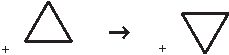
\includegraphics[width=1\textwidth,height=\textheight]{source/figures/shape_grammar_rule.pdf}
\caption{Örnek biçim grameri kuralı (Stiny, 2006).
\label{shapegrammarrule}}
\end{figure}

Biçim gramerleri görsel-mekansal düşünmeyi temsil eden bir biçimcilik
olarak da tanımlanabilmektedir. Görsel tasarım gramerleri olarak da
adlandırabileceğimiz biçim gramerleri dünyaya öğrenilen veya dayatılan
tanımlamalar yerine belirli bir zamanda pratik bir anlamı olan
tanımlamalardan bakabilme düşüncesidir (Özkar ve Stiny, 2009).

Tanıtımından sonra Gips (1975) doktora tezinde biçim gramerlerinin
bilgisayar uygulamalarını geliştirdi, Stiny (1975) ise matematiksel
temelleri üzerine yoğunlaştı. Stiny (1976) tezinin ardından yazdığı
\emph{Two exercises in formal composition} adlı makalede biçim
gramerlerinin kullanımını iki örnek üzerinden açıkladı ve bu örnekler
daha sonra yapılan çalışmalara temel oluşturdu. Bu örneklerden ilki
biçim gramerlerinin üretken bir sistem olarak yeni tasarım dili veya
tarzı oluşturmak için özgün hali ile nasıl kullanılabildiğini açıklarken
ikinci örnek ise mevcut bir tasarım dilinin veya tarzının biçim
gramerleri kullanılarak analizinin nasıl yapılabildiğini göstermektedir.
Ayrıca hem analitik hem de sentetik kullanıldığı örneklere de rastlamak
mümkündür (Knight, 1999).

\hypertarget{analiz-aracux131-olarak-kullanux131mux131-analiz-gramerleri}{%
\subsection{Analiz Aracı Olarak Kullanımı (Analiz
Gramerleri)}\label{analiz-aracux131-olarak-kullanux131mux131-analiz-gramerleri}}

Biçim gramerlerinin ilk kez analiz aracı olarak kullanımı Stiny (1977)
tarafından Çin buz ışını pencere tasarımları üzerine yaptığı çalışmada
ortaya konuldu. Bu çalışma ayrıca biçim gramerlerinin parametrik tasarım
ile entegre edilerek parametrik biçim gramerlerinin tanımlandığı çalışma
oldu. Beş adet kuraldan oluşan gramer Çin buz ışını ızgaraların bir
araya gelme düzenini açıklamayı, örnek ızgaralar oluşturmayı ve sayısız
yeni ızgara düzenleri oluşturmayı başardı. Ertesi yıl Stiny ve Mitchell
(1978) biçim gramerlerini Pallodio stili üzerinden test ederek ilk kez
bir mimari üslubun analizinde kullandılar. ``Palladio Grameri''
kurallarını Andrea Palladio tarafından 1570 yılında yazılmış
\emph{Quattro Libri dell'Architettura}'da bulunan villa planı
örneklerini inceleyerek tanımladılar. Parametrik biçim gramerlerini
kullanarak villaların zemin kat planlarını önerdikleri sekiz aşamalı bir
süreç ile oluşturdular.

Bu çalışmanın ardından gelen yirmi yıllık bir dönemde biçim gramerleri
neredeyse tamamen bir analiz aracı olarak mimarların tarzını, yöresel
mimariyi, sanat stillerini vb. açıklamada kullanıldı.

Bu çalışmalar arasında Giuseppe Terragni, Frank Lloyd Wright, Glenn
Murcutt, Christopher Wren gibi mimarların tarzları analiz edildi
(Flemming, 1981; Koning ve Eizenberg, 1981; Hanson ve Radford, 1986;
Buelinckx, 1993).

Yöresel mimari analizlerine bakıldığında Japon çay odaları, Buffalo'nun
bungalovları, Queen Anne evleri, geleneksel Tayvan evleri, geleneksel
Türk evleri, sıra evler, klasik Osmanlı dönemi camileri ve Mughul
bahçelerinin peyzaj mimarisi çalışmaları bulunmaktadır (Knight, 1981;
Downing ve Flemming, 1981; Flemming, 1987; Chiou ve Krishnamurti, 1995;
Çağdaş, 1996; Çağdaş, 1996; Aksoy, 2001; {\textbf{???}}).

Sanat stillerinin analizini yapan çalışmalarda Richard Diebenkorn,
Georges Vantongerloo ve Fritz Glarner'ın tabloları, Hepplewhite tarzı
sandalyelerin arkalıklarının tasarımı, Frank Lloyd Wright'ın pencere
tasarımları ve antik Yunan çömleklerinin süsleme tasarımları
incelenmiştir (Kirsch ve Kirsch, 1986; Knight, 1989; Knight, 1980;
Rollo, 1995; Knight, 1986). Wright'ın mimari tarzı için hazırlanan
gramer ilk üç boyutlu mimari gramer çalışması olması açısından
önemlidir.

Sonraki dönem çalışmalarında Benros vd. üç ayrı tarz olan Pallodio
villaları, Malagueira konutları ve Prairie konutlarını oluşturdukları
tek gramer, Osmanlı camilerinin ontolojisini kullanan tipolojik
tanımlama (description) gramerleri ve tipolojik tanımlama gramerleri
için genel gösterim önerisi göze çarpmaktadır (Benrós vd., 2014; Stouffs
ve Tunçer, 2015; Stouffs, 2016).

\hypertarget{tasarux131m-aracux131-olarak-kullanux131mux131-uxf6zguxfcn-gramerler}{%
\subsection{Tasarım Aracı Olarak Kullanımı (Özgün
Gramerler)}\label{tasarux131m-aracux131-olarak-kullanux131mux131-uxf6zguxfcn-gramerler}}

Biçim gramerlerinin analiz aracı olarak kullanımı yukarıdaki örneklere
bakıldığında önemli ölçüde etkin olduğunu göstermektedir. Buna karşı
başlangıçtan itibaren tamamen yeni tasarım dilleri oluşturma konusunda
şaşırtıcı bir şekilde sınırlı sayıda örneğe rastlanmaktadır. Bu anlamda
ilk çalışma Stiny ve Gips (1972) tarafından tablolar üzerine yapılan
biçim gramerleri oldu. Stiny ve Gips'in tezleri ve beraber yazdıkları
\emph{Algorithmic Aesthetics} kitabı da yine aynı konu üzerinde biçim
grameri formalizmini örnekliyordu (Knight, 1999).

Bu çalışmalar haricinde Stiny'nin (1976) iki boyutlu formal
kompozisyonlar ve ilk üç boyutlu biçim grameri çalışması olan Froebel'in
yapı blokları üzerine çalışmaları örnek oluşturmaktadır (Stiny, 1980).
Froebel yapı blokları üzerine olan çalışma özgün gramerleri kullanarak
sıfırdan yeni bir tasarım dili oluşturmak için izlenecek işleyişi
tanımlamaktadır. Yeni tasarım dilini oluşturmak için önerilen işleyişte
biçim sözlüğü, mekansal ilişkiler, biçim kuralları, başlangıç biçimi ve
biçim gramerlerinin aşamalı olarak oluşturulması gerekmektedir. Bu
alanda mimarlık ve diğer dallarda çeşitli çalışmalar kısıtlı sayıda
gerçekleştirildi (Knight, 1989; Knight, 1992; Knight, 1993; Knight,
1994).

\hypertarget{analiz-sonucu-tasarux131m-aracux131-olarak-kullanux131mux131-hibrid-gramerler}{%
\subsection{Analiz Sonucu Tasarım Aracı Olarak Kullanımı (Hibrid
Gramerler)}\label{analiz-sonucu-tasarux131m-aracux131-olarak-kullanux131mux131-hibrid-gramerler}}

Özgün gramelerin tamamen baştan oluşturulması teori üzerinde olmaktadır
(Knight, 1999). Uygulamada ise yeni tasarım dilleri eski ve güncel
dillerin değiştirilmesi, geliştirilmesi veya birleştirmesi gibi işlemler
ile oluşturulur. Knight (1981) önerdiği mevcut tasarım dilleri üzerinden
yeni tasarım dilleri üretme yönteminde ilk önce mevcut dil için bir
gramer çıkartılarak analiz edilir, çıkarılan gramerin kuralları
dönüştürülür ve dönüştürülen kurallar yeni bir gramerin ve dilin temeli
haline gelir. Knight bu yöntemin bilinen dillerin tarihsel evrimini
başarılı bir şekilde tanımlamak ve yeni tasarımlar geliştirmek için
kullanabileceğini belirtmektedir. Bu nedenle bu yöntem hem analitik hem
sentetiktir. Knight \emph{Transformations in Design} adlı kitabında bu
yöntemi kullanarak Frank Lloyd Wright'ın çalışmalarında, De Stijl
resminde ve antik Yunan süsleme tasarımlarında stilistik değişimleri
analiz etmek için uygulamaktadır (Knight, 1999). Flemming (1990)
Knight'ın yöntemine benzer bir yöntemi bilgisayar üzerinde mimari
kompozisyonları öğretebilmek için kullanmmıştır.

Bu gramer yapısının örneklerine baktığımızda Çolakoğlu (2001) 18. ve 19.
yüzyılda Saraybosna'da Osmanlı tarzında tasarlanan geleneksel ``Hayat''
evlerinin gramerini oluşturarak tarihi bağlama uygun yeni formların
üretimini sağladı. Duarte (2005) 1977 ve 1996 yılları arasında Siza
tarafından Malagueira için tasarlanmış otuzbeş konut üzerinden Siza'nın
da desteğini alarak oluşturduğu gramer ile Siza'nın tasarım mantığına
yatkın çeşitli yeni tasarımlar üretebildi. Marakeş Medine'de Zaouiat
Lakhdar bölgesi için geliştirilen yerel konut ve kentsel form üreten
gramerler, \emph{rabo-de-bacalhau} bina tipolojisindeki evlerin
rehabilitasyonu için geliştirilen dönüşüm grameri hibrid gramerlere
örnek oluşturmaktadır (Duarte ve Rocha, 2006; Duarte vd., 2007; Eloy ve
Duarte, 2014).

\hypertarget{split-grameri}{%
\subsection{Split Grameri}\label{split-grameri}}

Wonka vd. (2003) mimari modelleri oluşturmak için özel bir set
grameri\footnote{(Stiny, 1982)}olan parametrik split gramer yöntemini
geliştirmişlerdir. Yazarlar yapıların yatayda ve düşeyde sürekliliğe
sahip olan yapı elemanlarından oluştuğunu ve buna benzer bir etkiyi
split grameri kontrol ederek elde edilebileceğini belirtmişlerdir.
İsmini bölümleme işleminden alan ve iki üretim kuralı olan bu yöntem
basit geometrilerden oluşan üç boyutlu bir kütlenin önce yüzeylere ve
yapısal elemanlarına kadar bölümlenip ardından bölümlenen her biçim
önceden tanımlanan geometri ve malzemeler ile yer değiştirmesine
dayanmaktadır (Şekil \ref{splitGrammar}). Bölümlenme işlemi sonlandırıcı
tanımlı biçimlere ulaşana kadar devam etmektedir ve muhtemel düzeni
önceden tanımlı-sabit olduğundan dolayı kararlıdır.

\begin{figure}
\centering
\includegraphics[width=1\textwidth,height=\textheight]{source/figures/splitGrammar.pdf}
\caption{Basit bir Split Gramer kuralı ve üretim süreci.
\label{splitGrammar}}
\end{figure}

Set grameri üretim kurallarını görsel işlem yerine etiketli biçimler
üzerinden işleyen, biçim gramerlerinin basitleştirilmiş halidir (Stiny,
1982; Lienhard, 2017). Etiketli bir biçim set gramerinin en küçük
(atomik) öğesidir ve alt biçimler barındırmaz. Etiketler sembol olarak
kullanılarak üretim kurallarının metinsel olarak yazımını ve
bilgisayarda algoritma olarak işlenmesine olanak vermektedir. İdeal
olarak, bir biçim grameri uygulaması: görsel bilgi işlemeyi
desteklemeli, saklı şekillere izin vermeli (emergence), önceden
tanımlanmış parçalara dayanmamalı ve parametrik olmalıdır (Gips, 1999).
Set gramerleri biçim gramerlerinin bilgisayar üzerinde işlenmesini
kısıtlayan ilk üç özelliğini barındırmamaktadır. Literatürde biçim
grameri uygulaması olarak adlandırılan bir çok yazılım ve yazılım
denemesi aslında set gramerini temel alarak çalışmaktadır.

\hypertarget{cga-biuxe7im-grameri}{%
\subsection{CGA Biçim Grameri}\label{cga-biuxe7im-grameri}}

Split gramerler Müller vd. (2006) tarafından geliştirilerek CGA
gramerleri olarak adlandırılmıştır. Geliştirilen bu yöntemde katı kütle
modelleme sistemi ve farklı olarak tanımlanmış birçok modelleme
kuralının yanında cephe üretimi zor olan karmaşık kütleler içinde
eklentiler bulunmaktadır. CGA gramer yöntemi çokgen ile belirlenmiş bir
parsel hattını yükseltip katlara bölünmüş bir hacim oluşturarak işleme
başlamaktadır. Katların cepheleri biçim kuralları kullanılarak duvar,
kapı, pencere gibi bölümlere bölünmektedir. Koşullu ya da tahmini
kurallar, biçim parametreleri, rastgele numara üretimi bu yöntem
içerisinde çeşitlilik oluşturmak için kullanılmaktadır. CGA bir biçim
grameri olması ile beraber aynı zamanda bir programlama dilidir. Örnek
bir CGA biçim kuralı aşağıdaki gibi yazılmaktadır.

\begin{verbatim}
başlangıçŞekli -->
                    koşul1: sonuçŞekil0 ... sonuçŞekilM ...
                    koşulN: ...
\end{verbatim}

CGA gramerlerinin tanımlanmasının ardından yordamsal modellemenin
kolaylaştırılması ve daha iyi kullanılabilmesi için devamlı gelişmeler
gözlendi. Özellikle cephe modelleri oluşturmak için Müller vd. (2007)
binaların cephe fotoğrafları üzerinden tekrar eden karoların
tanımlanması ile gramer kurallarınının bilgisayar tarafından otomatik
çıkarılması için bir yöntem geliştirdi. Lipp vd. (2008) CGA kurallarını
kod yazarak oluşturmak yerine yaptıkları yazılım sayesinde üç boyutlu
model üzerinden etkileşim ile kodları görsel olarak düzenlemeyi
başardılar. Ancak bu gelişmelere rağmen birçok yordamsal modelleme
projesi kod yazılarak gerçekleştirildi. Bunlardan bazıları;

\begin{itemize}
\tightlist
\item
  Reconstruction of Puuc Buildings (Müller vd., 2006)
\item
  Reconstruction of Ancient Pompeii (Müller vd., 2005)
\item
  Rome Reborn 2.0: A Case Study of Virtual City Reconstruction Using
  Procedural Modeling Techniques (Dylla vd., 2010)
\item
  Urban Topography of Magnesia on the Maeander (Knight, 2016).
\end{itemize}

\hypertarget{uxe7alux131ux15fma-alanux131nux131n-seuxe7imi}{%
\section{Çalışma Alanının
Seçimi}\label{uxe7alux131ux15fma-alanux131nux131n-seuxe7imi}}

Kentsel gelişim sürecinde kent kimliği hayati bir öneme sahiptir.
Küreselleşmenin de etkisiyle şehirler gelişim ve dönüşüm süreçlerinde
özgün kimliklerini kaybetme problemiyle karşılaşmaktadır. Bu gelişim ve
dönüşüm süreçleri düzgün işletilemediğinde kent okunabilirliğini,
kentliler kent hafızasını ve algısını kaybetmektedir. Bu durum kentin
tarihi ve kültürel mirasını korumayı güçleştirmektedir.

Ekonomik, sosyal, teknolojik, kültürel değişimler ve yanlış planlama
kararları sonucunda Trabzon kenti tarihi kent dokusunda tahribatlara ve
kimlik kaybetme tehlikesine maruz kalmıştır. Kentin bir çok bölgesinde,
kentsel sit alanları da dahil olmak üzere, bu tahribat ve kayıplar
yaşanmakta ve geleneksel konut mirasına ait ürünler gün geçtikçe
azalmaktadır.

Bu bağlamda Trabzon kentinin geleneksel dokusuna ait karakteristik
örnekleri bir arada bulunduran ve tarih boyunca kent çekirdeğinin
biçimlendiği bölge olan Ortahisar mahallesi çalışma alanı olarak
seçilmiştir. Çalışma bu bölgedeki geleneksel konut karakterine ait
bilgileri yordamsal modelleme yöntemi için gerekli CGA grameri ile kayıt
altına almayı ve bölgede yapılması planlanan yeni yapılar için tasarım
altlığı oluşturmayı hedeflemektedir.

\hypertarget{uxe7alux131ux15fma-alanux131na-iliux15fkin-bilgiler}{%
\section{Çalışma Alanına İlişkin Bilgiler
}\label{uxe7alux131ux15fma-alanux131na-iliux15fkin-bilgiler}}

\begin{figure}
\centering
\includegraphics[width=1\textwidth,height=\textheight]{source/figures/TrabzonTurkiye.png}
\caption{Türkiye'de Trabzon'un konum haritası.}
\end{figure}

Trabzon Doğu Karadeniz sahil şeridinde doğal bir liman olan Asya ve
Ortadoğu transit yolunun başında kurulmuştur. Liman ve ticaret kenti
olarak özellikle 7. yüzyıldan sonra ekonomik anlamda bölgenin önemli
merkezi olmuştur . Kuzeyde Karadeniz, doğu ve batıda ise derin vadiler
ile çevrili kent coğrafi olarak korunaklı bir bölgede
konumlandırılmıştır. Güney kısmında doğal bir sınırının olmaması ve
savunma ihtiyacından ötürü kent önce Yukarıhisar diye adlandırılan
güneydeki en yüksek kısmından başlanarak kuzeye doğru sırayla Ortahisar
ve Aşağı hisar kısımlarının inşaa edildiği söylenebilir (Uspenski,
2003).

\begin{figure}
\centering
\includegraphics[width=1\textwidth,height=\textheight]{source/figures/TrabzonMap.png}
\caption{Ortahisar bölgesinin kentin 1223 yılı öncesi ve 1869 yılına
kadar olan tarihlerde konumunu gösteren harita (Bryer ve Winfield,
1985).}
\end{figure}

Çalışma alanı olarak seçilen Ortahisar, Zağnos ve Tabakhane vadileri
arasında kalan, Trabzon kentinin tarihi çekirdeğinin bulunduğu yerleşim
bölgesidir. Mimari yapı kültürü M.Ö. 7. yüzyıla kadar dayanmaktadır ve
tarih boyunca kentin idari, dini ve yaşam merkezi olarak hizmet etmiştir
(Tuluk ve Düzenli, 2010). Tarihi surlar ile çevrelenmiş bölge, farklı
dönemlere ait geleneksel sivil mimari örneklerinin yanında anıtsal
yapıları da barındırmaktadır. Günümüze ulaşmış Ortahisar sınırları
içinde kalan sivil mimari dışındaki önemli yapılar aşağıdaki listede
sıralanmıştır.

\begin{itemize}
\tightlist
\item
  Askeri Mimari

  \begin{itemize}
  \tightlist
  \item
    Kent surları
  \end{itemize}
\item
  Dini Mimari

  \begin{itemize}
  \tightlist
  \item
    Panaghia Chrysokephalos Kilisesi (Ortahisar veya Büyük Fatih Cami)
  \item
    Musa Paşa Cami
  \item
    Ortasaray Mescidi - Saraçzade Medresesi
  \item
    Şirin Hatun Mescidi
  \end{itemize}
\item
  Endüstriyel Mimari

  \begin{itemize}
  \tightlist
  \item
    Tabakhane Köprüsü
  \item
    Zağnos Köprüsü
  \end{itemize}
\item
  Su Mimarisi

  \begin{itemize}
  \tightlist
  \item
    Çifte Hamam
  \item
    Çarıkçı-Zade Hacı İsmail Çeşmesi
  \item
    Çeşme (Ortahisar Cami güneyinde)
  \end{itemize}
\item
  Kamusal Mimari

  \begin{itemize}
  \tightlist
  \item
    Hüseyin Kazaz Kültür Merkezi (Eski Cezaevi Binası)
  \item
    Trabzon Kültür Müdürlüğü (Eski Hükümet Konağı)
  \item
    Gazi Paşa İlköğretim Okulu
  \end{itemize}
\end{itemize}

\begin{figure}
\centering
\includegraphics[width=1\textwidth,height=\textheight]{source/figures/DiniMimari.png}
\caption{Ortahisar dini mimari örnekleri. Solda Ortahisar Cami ve sağda
yıkılmış Şirin Hatun Mescidi (Özen vd., 2009).}
\end{figure}

\begin{figure}
\centering
\includegraphics[width=1\textwidth,height=\textheight]{source/figures/EndustriyelMimari.png}
\caption{Ortahisar endüstriyel mimari örnekleri. Solda Tabakhane Köprüsü
ve sağda Zağnos Paşa Köprüsü. Kaynak: www.eskiturkiye.net}
\end{figure}

\begin{figure}
\centering
\includegraphics[width=1\textwidth,height=\textheight]{source/figures/SuMimarisi.png}
\caption{Ortahisar su mimarisi örnekleri. Solda yıkılmış Çifte Hamam ve
sağda Ortahisar Cami güneyindeki çeşme (Özen vd., 2009).}
\end{figure}

\begin{figure}
\centering
\includegraphics[width=1\textwidth,height=\textheight]{source/figures/KamusalMimari.png}
\caption{Ortahisar kamusal mimari örnekleri. Solda Hüseyin Kazaz Kültür
Merkezi ve sağda Trabzon Kültür Müdürlüğü binası (Özen vd., 2009).}
\end{figure}

Listelenmiş yapılardan kent surlarının yapım tarihi net olarak
bilinmemekle beraber 257 yılından önce mevcut olduğu kaynaklarda
belirtilmiştir (Bryer ve Winfield, 1985). Surlardan sonra bölgedeki en
eski yapı olan ve Ortahisar Cami olarak adlandırılan Panaghia
Chrysokephalos Kilisesi 914 yılında inşa ettirilmiştir (Miller, 2007).
Bölgedeki diğer anıtsal yapıların inşa tarihleri 13. ve 16. yüzyıl,
sivil mimarlık örneklerinin inşa tarihlerinin ise 19. yüzyıl sonları ve
20. yüzyılın ilk çeyreği olduğu bilinmektedir (Aysu, 1977; Kuloğlu,
1994; Tuluk ve Düzenli, 2010). Mevcut yapıların korunması ve yeni
yapıların sınırlandırılması amacıyla bölge 1985 yılında 2 Nolu Ortahisar
Kentsel Sit Alanı olarak tescillenmiştir.

\begin{figure}
\centering
\includegraphics[width=1\textwidth,height=\textheight]{source/figures/ortahisar.jpg}
\caption{Ortahisar'ın yeni kent merkezine göre konumunu gösteren harita
(Var, 2015).}
\end{figure}

\begin{figure}
\centering
\includegraphics[width=1\textwidth,height=\textheight]{source/figures/OrtahisarUyduIzli.jpg}
\caption{Ortahisar uydu fotoğrafı.}
\end{figure}

1938 yılında Jacques H. Lambert tarafından hazırlanan Trabzonun ilk imar
planı Ortahisar bölgesinin mevcut yapıları ile beraber olduğu gibi
korunmasını önermiştir. 1968 yılında açılan yarışma ile başlayan ikinci
planlama çalışmalarında da kentin eski yerleşkelerinin korunması
hedeflenmiştir. Bu çalışmalarda şehrin genişleyebilmesi için
Ortahisar'ın güney kısmından teğet geçmesi önerilen Tanjant Yolu 2002
yılında surlar üzerinden ve tarihi kent merkezini ortasından ikiye
ayıracak şekilde uygulamaya konulmuştur. Bu değişiklik bölge dokusunda
yıkımlara ve büyük tahribata sebep olmuştur.

\hypertarget{ortahisar-konutlarux131nux131n-uxf6zellikleri}{%
\subsection{Ortahisar Konutlarının
Özellikleri}\label{ortahisar-konutlarux131nux131n-uxf6zellikleri}}

Ortahisar'da bulunan geleneksel konutlar yaklaşık bir asır öncesine
dayanan tarihleriyle ağırlıklı olarak Osmanlı dönemine ait yapılardır.
Yapım malzemesi ve teknolojisinin imkan verdiği koşullar ile ahşap-kagir
yapılar 2-2,5 kat, taş yığma yapılar 3-3,5 kat olarak inşa
edilmiştirler. Belli bir geometrik düzeni olmayan parseller içinde olan
geleneksel konut dokusu;

\begin{itemize}
\tightlist
\item
  Surlara yakın veya üzerinde, veya bir duvarı ya da terası surların bir
  parçası olarak
\item
  Kuzey güney aksında bitişerek gelişmiş ve vadilere yönelmiş
\item
  Yoldan yüksek duvarlarla soyutlandırılan bahçe-avlu karışımı bir
  alandan geçilerek oluşturulmuş konut grubu
\item
  Parsel sınırları içinde yönlere ve kullanışlara göre bir veya iki
  kenarı parsel sınırına ya da komşu binaya dayanarak geliştirilmiş
  konut grubu şeklinde bir araya gelmişlerdir. 
\end{itemize}

Ortahisar konutları plan şeması olarak karnıyarık diye adlandırılan iç
sofalı düzenlemeye sahiptirler. Az sayıda da olsa dış sofalı plan şeması
örnekleri de bölgede bulunmaktadır. İç sofalı plana sahip evlerde
çıkmalı ve çıkmasız olarak örnekleri varken, dış sofalı konutlarda açık
ve kapalı olma durumları söz konusudur (Birlik, 1999).

\begin{figure}
\centering
\includegraphics[width=1\textwidth,height=\textheight]{source/figures/SofaliPlanlar.jpg}
\caption{Çıkmalı ve çıkmasız iç sofa örnekleri olarak Nilay Soley ve
Resul Özerk evleri (Özen vd., 2009).}
\end{figure}

\begin{figure}
\centering
\includegraphics[width=1\textwidth,height=\textheight]{source/figures/disSofaliPlanlar.jpg}
\caption{Açık ve kapalı dış sofa örnekleri olarak Bekir Gerçek ve Salih
Türkmen evleri (Kuloğlu, 1994).}
\end{figure}

Geleneksel dokuda ve çevresinde bulunan mimari örnekler yapım dönemine
göre bazı özelliklerinde farklılıklar göstermektedir. Ancak Fallmerayer
(2011) Ortahisar konutları için Bizans'a bağlı Komnenos Hanedanlığı
döneminden itibaren mimari üslup bakımından değişime uğramadığını hatta
ölçü ve yönlenme gibi özelliklerinin de değişmediğini belirtmektedir.
Yapı stoğu incelendiğinde bölgede Rum dönemi, Osmanlı dönemi, Cumhuriyet
sonrası dönem olmak üzere üç döneme ait yapılara rastlanmaktadır. Rum ve
Osmanlı dönemi yapıları birbirlerinden yapı malzemesi kullanımında
ayrışmaktadır. Rum dönemi yapıların inşaasında yapı malzemesi olarak
genellikle taş kullanılırken Osmanlı dönemi yapılarında ağırlıklı olarak
ahşap kullanılmıştır. Osmanlı dönemi ve önceki dönemlerin benzer
özellikleri;

\begin{itemize}
\tightlist
\item
  Cephe;

  \begin{itemize}
  \tightlist
  \item
    Yapı cepheleri genel olarak yatayda ve düşeyde simetriktir,
  \item
    Cephede köşe noktalarda düşey, kat aralarında yatay bantlar
    kullanılmıştır,
  \item
    Cephede açık ve kapalı çıkmalar görülmektedir, bu çıkmalar iç
    mekanda bulunan oda veya sofa genişliğindedir,
  \item
    Cepheler sokağa paraleldir,
  \item
    Beşik çatı ve ağırlıkla kırma çatı tipi hakimdir,
  \item
    Zemin katlar su basman seviyesinde yükseltilerek bodrum katların
    aydınlatılması için pencereler kullanılmaktadır,
  \end{itemize}
\item
  Giriş;

  \begin{itemize}
  \tightlist
  \item
    Genellikle cephenin simetri ekseninde, diğer durumlarda yapının
    köşesine yakın bulunurlar,
  \item
    Basamaklar ve hemen üzerindeki çıkmalar ile vurgulanmışlardır,
  \end{itemize}
\item
  Pencereler;

  \begin{itemize}
  \tightlist
  \item
    Dikdörtgen formda ve düşey hatlıdırlar,
  \item
    Sokak cephesinde diğer cephelere göre daha çok pencere
    bulunmaktadır.
  \end{itemize}
\end{itemize}

\begin{figure}
\centering
\includegraphics[width=1\textwidth,height=\textheight]{source/figures/KonutCepheleri.jpg}
\caption{Geleneksel konut cephesi örnekleri. Solda İsmail Taşkın evi
sağda Mustafa Saltoğlu evi (Özen vd., 2009).}
\end{figure}

Cumhuriyet sonrası dönem yapıları kargir-yığma ve betonarme olarak inşaa
edilmişlerdir (Kuloğlu, 1994). Osmanlı dönemi sonrası yapılan bu yapılar
hızlı gelişen ekonomik, sosyal, teknolojik ve kültürel değişimlerin
sonucu olarak geleneksel dokuya uyum sağlayamamıştır.

\hypertarget{verilerin-toplanmasux131}{%
\section{Verilerin Toplanması}\label{verilerin-toplanmasux131}}

Ortahisar geleneksel konutlarına ait bilgiler rölövelerden, akademik
çalışmalardan ve alan üzerine yazılmış kitaplardan elde edilmiştir.
Konutlara ait rölöveler iki arşivden derlenerek gramer için örneklem
kümesi oluşturulmuştur. Örneklem kümesi geleneksel Ortahisar
konutlarının hepsini içermemektedir; ancak değişik özelliklere sahip
yapıları barındırmaktadır.

Çalışma alanı içerisinde 73 adet tescilli yapı bulunmaktadır. Bunlardan
25 adet tescilli yapının rölöveleri Trabzon Büyükşehir Belediyesi
arşivlerinden ve Trabzon Rölöve ve Anıtlar Müdürlüğü arşivlerinden elde
edilen veriler bir araya getirilerek derlenmiştir. Ortahisar
bölgesindeki tescilli yapılar ve rölövelerine ulaşılabilen tescilli
yapılar şekil \ref{ortahisartescilli}'te gösterilmiştir. Arka planı koyu
renkli olan yapılar rölövelerine ulaşılabilenleri ifade etmektedir.

\begin{figure}
\centering
\includegraphics[width=1\textwidth,height=\textheight]{source/figures/vaziyetplanitescilli.pdf}
\caption{Ortahisar bölgesi tescilli yapılarını gösteren vaziyet planı.
\label{ortahisartescilli}}
\end{figure}

Trabzon Büyükşehir Belediyesi arşivlerinden Trabzon Büyükşehir
Belediyesi ve Bimtaş A.Ş. tarafından 2012 yılında Ortahisar'da LIDAR
teknolojisi kullanılarak yapılan çalışmadan bölgenin sokak silüetleri
elde edilmiştir. Sokak silüetlerinden bazı yapıların sadece tek
cepheleri elde edilebilmiş ve geri kalan cephelerinin rölövelerine
ulaşılamamıştır. Bir kısmı ise tescilli olmasına rağmen geleneksel
dokuyu yansıtmadığından dolayı çalışmaya katılmamıştır.

\begin{figure}
\centering
\includegraphics[width=1\textwidth,height=\textheight]{source/figures/Corpus.pdf}
\caption{Grameri oluşturan yapı tiplerinin örneklem kümesi.
\label{orneklemkumesi}}
\end{figure}

Çalışma kapsamında incelenen 15 adet yapı 19. yüzyılın ikinci yarısı ve
20. yüzyılın ilk çeyreği arasındaki dönemde yapılmıştırlar. Bunlar
arasından 118 ada 1 parsel ve 128 ada 10 parselde bulunan konutlar yakın
tarihte betonarme olarak yeniden inşa edilmiş yapılardır.

Örneklem kümesindeki yapılar şekil \ref{orneklemkumesi}'te yapı tipine
göre sınıflandırılarak gösterilmiştir. Yapılar ilk olarak cephe tipine
göre bir parçalı ve üç parçalı cepheye sahip olarak ikiye ayrılmaktadır.
Yapıların bir parçalı ve üç parçalı cepheye göre sınıflandırılması ön ve
arka cephelerindeki pencere dizilimi ve kapalı veya açık çıkmasına bağlı
olarak gerçekleşmektedir. Ardından yapılar kat sayısına, çıkma tipine,
giriş katlarına göre şekil içerisinde gruplandırılmıştır. Açık tonda
taramalar yapıların giriş katlarını ifade etmektedir.

Yapılara ait rölöve çizimleri ve künye bilgileri her bir yapı için
oluşturulan yapı bilgi formlarında düzenlenmiştirler. 110 ada 16
parselde bulunan yapıya ait örnek yapı bilgi formu şekil
\ref{yapibilgiformu}'da gösterilmiştir. Yapı bilgi formları ekler
kısmında bulunmaktadır.

\begin{figure}
\centering
\includegraphics[width=1\textwidth,height=\textheight]{source/figures/BilgiFormlari/110-16.pdf}
\caption{Yapı bilgi formu örneği. \label{yapibilgiformu}}
\end{figure}

Düzenlenen rölöve verileri içerisinden gerekli ölçüler her eleman için
dış hizaları temel alınarak ölçülmüştür. Örneğin pencere ve kapılar
söveleri ile beraber tek bir ünite şeklinde ölçülerek hesaplara dahil
edilmiştirler. 110 ada 16 parsel ve 39 parsele ait yapıların ön
cephelerinin ölçülendirilmiş halleri şekil \ref{roloveoran}'de
gösterilmiştir. Elde edilen verilerin incelenmesinin ardından geleneksel
konutlar hakkında ortaya çıkan önemli bilgiler bir sonraki bölümde ele
alınarak vurgulanmıştır.

\begin{figure}
\centering
\includegraphics[width=0.9\textwidth,height=\textheight]{source/figures/RoloveOranlar.pdf}
\caption{110 ada 16 ve 39 parsellerdeki yapılara ait rölövelerin
ölçülendirilmiş gösterimleri. \label{roloveoran}}
\end{figure}

\newpage

\hypertarget{bulgular-ve-irdelemeler}{%
\chapter{BULGULAR VE İRDELEMELER}\label{bulgular-ve-irdelemeler}}

\thispagestyle{empty}

Bu bölümde elde edilen rölöveler üzerinden yapılan analizler ve bunların
CGA kodunun oluşturulmasındaki kullanımı anlatılmaktadır. CGA gramerinin
oluşturulmasında sırasıyla binaların;

\begin{itemize}
\tightlist
\item
  Taban alanları
\item
  Kat sayıları ve yükseklikleri
\item
  Cephe tipi
\item
  Cephe çıkmaları
\item
  Cephe elemanları
\item
  Çatı formu
\end{itemize}

analiz edilerek incelenmiştir. Bu analizlere ek olarak yapıların
kütlesel formları gruplanarak analiz edilmiştir. Ardından bu formları ve
türevlerini oluşturabilecek biçim grameri kuralları tanımlanmıştır. Bu
kurallar CGA gramerine entegre edilerek kaba kütle üretimi sağlanmaya
çalışılmıştır.

Oluşturulan kütleler kat sayıları ve yükseklik oranlarına göre
dilimlenerek katlar oluşturulmaktadır. Cephe karakteri analizi sonucunda
ise oluşan katların panel parçalarına ayrılması sağlanmaktadır. Ardından
cephe elemanları ve pencereler oranlarına göre panel içinde dilimlenerek
yerleri belli edilmektedir.

\hypertarget{ortahisarux131n-mimari-dil-analizi-ve-biuxe7im-grameri}{%
\section{Ortahisar'ın Mimari Dil Analizi ve Biçim
Grameri}\label{ortahisarux131n-mimari-dil-analizi-ve-biuxe7im-grameri}}

Gramer kuralları iki boyutlu bina oturum alanı ve üç boyutlu bloklardan
oluşmaktadır. CGA gramerinin başlangıcı bir parsel veya bina oturum
alanının tanımlanması ile gerçekleşmektedir. Üç boyutlu bloklar kütlesel
hacimlere karşılık gelmekte ve analiz-sentez aşaması sonucunda elde
edilen veriler ile parametreleştirilmektedir. Gramerin basitleştirilmesi
açısından parametre değer verileri ayrıca tablolar ile açıklanmıştır.

Çalışmanın amacı geleneksel konutların oranlarını üretebilen tasarım
altlığı oluşturabilmek olduğu için cephelerdeki bir kural tanımlamayan
düzensizlikler göz ardı edilmiştir. Amaç birebir varolan yapıları
üretmek değil onların oranlarını gösteren modeller üretebilmektir.

Analiz edilen yapıların kendi içlerinde ve birbirleri ile
karşılaştırılan yükseklik değerleri arasında bir korelasyon
bulunamadığından yükseklikler zemin kat yüksekliği sabit alınarak
orantılanmıştır.

\hypertarget{yapux131-taban-alanux131}{%
\subsection{Yapı Taban Alanı}\label{yapux131-taban-alanux131}}

Ortahisar geleneksel evleri sokağa göre paralel konumlanmaktadır.
Yapıların giriş ve kapalı çıkmasının bulunduğu cephe sokağa doğru
bakmaktadır. Kural 1 ve 2 başlangıç için verilen oturum alanını ve
sokağın yönünü belirler (Şekil \ref{K1K2}). Kural 1 herhangi bir alanın
bir noktasında oturum alanını konumlandırmak için kullanabileceğinden
alan planlamasını mümkün kılmaktadır.

\begin{figure}
\centering
\includegraphics[width=1\textwidth,height=\textheight]{source/figures/K1-K2.pdf}
\caption{Oturum alanı ve sokak yönünün tanımlanmasını gösteren kurallar.
\label{K1K2}}
\end{figure}

Seçilen Ortahisar evlerinin taban alanları incelendiğinde;

\begin{itemize}
\tightlist
\item
  En küçük yapı taban alanı : 50,38 m\textsuperscript{2}
\item
  En büyük yapı taban alanı : 315,67 m\textsuperscript{2}
\item
  En kısa kenar uzunluğu : 4,888 m
\item
  En uzun kenar uzunluğu : 17,021 m
\item
  Plan derinliğinin genişliğine oranının en küçük değeri 0,346 en büyük
  değeri 1,513
\end{itemize}

oldukları bulunmuştur. Bulunan değerler CGA gramerine girdi olarak
verilen taban alanlarının seçimi için kullanılmaktadır. Bu kısıtlar
dışında olan girdilerde model oluşumu gerçekleşmemektir. \newpage

\begin{longtable}[]{@{}rrrrrrr@{}}
\caption{Seçilmiş Ortahisar evlerinin oturum alanları, ortalama derinlik
ve ortalama genişlik değerleri tablosu.
\label{EvlerAlanlarOrtalamalar}}\tabularnewline
\toprule
\textbf{Ada} & \textbf{Parsel} & \textbf{Ort. Derinlik} & \textbf{Ort.
Genişlik} & \textbf{Der. / Gen.} & \textbf{Taban Alanı} & \textbf{Parsel
Alanı}\tabularnewline
\midrule
\endfirsthead
\toprule
\textbf{Ada} & \textbf{Parsel} & \textbf{Ort. Derinlik} & \textbf{Ort.
Genişlik} & \textbf{Der. / Gen.} & \textbf{Taban Alanı} & \textbf{Parsel
Alanı}\tabularnewline
\midrule
\endhead
\textbf{110} & \textbf{16} & 7,955 m & 12,628 m & 0,630 & 100,43
m\textsuperscript{2} & 191,09 m\textsuperscript{2}\tabularnewline
\textbf{110} & \textbf{23} & 5,012 m & 10,067 m & 0,498 & 50,38
m\textsuperscript{2} & 84,07 m\textsuperscript{2}\tabularnewline
\textbf{110} & \textbf{39} & 12,678 m & 16,048 m & 0,790 & 194,83
m\textsuperscript{2} & 890,45 m\textsuperscript{2}\tabularnewline
\textbf{110} & \textbf{41} & 8,528 m & 14,385 m & 0,593 & 117,90
m\textsuperscript{2} & 320,49 m\textsuperscript{2}\tabularnewline
\textbf{110} & \textbf{43} & 12,501 m & 8,320 m & 1,503 & 110,31
m\textsuperscript{2} & 124,59 m\textsuperscript{2}\tabularnewline
\textbf{110} & \textbf{44} & 10,284 m & 8,165 m & 1,259 & 74,16
m\textsuperscript{2} & 45,80 m\textsuperscript{2}\tabularnewline
\textbf{110} & \textbf{131} & 6,670 m & 13,247 m & 0,503 & 93,91
m\textsuperscript{2} & 1.639,41 m\textsuperscript{2}\tabularnewline
\textbf{114} & \textbf{30} & 10,975 m & 7,255 m & 1,513 & 100,23
m\textsuperscript{2} & 131,28 m\textsuperscript{2}\tabularnewline
\textbf{118} & \textbf{1} & 9,208 m & 14,904 m & 0,618 & 137,30
m\textsuperscript{2} & 177,17 m\textsuperscript{2}\tabularnewline
\textbf{127} & \textbf{28} & 8,473 m & 9,799 m & 0,865 & 83,43
m\textsuperscript{2} & 205,86 m\textsuperscript{2}\tabularnewline
\textbf{128} & \textbf{7} & 8,473 m & 10,102 m & 0,839 & 92,20
m\textsuperscript{2} & 180,38 m\textsuperscript{2}\tabularnewline
\textbf{128} & \textbf{10} & 4,888 m & 14,111 m & 0,346 & 61,41
m\textsuperscript{2} & 102,06 m\textsuperscript{2}\tabularnewline
\textbf{129} & \textbf{26} & 16,493 m & 15,992 m & 1,031 & 242,79
m\textsuperscript{2} & 203,24 m\textsuperscript{2}\tabularnewline
\textbf{888} & \textbf{7} & 15,746 m & 12,945 m & 1,216 & 199,34
m\textsuperscript{2} & 603,81 m\textsuperscript{2}\tabularnewline
\textbf{888} & \textbf{8} & 14,998 m & 17,021 m & 0,881 & 315,67
m\textsuperscript{2} & 879,21 m\textsuperscript{2}\tabularnewline
\bottomrule
\end{longtable}

\hypertarget{yapux131-kat-sayux131sux131-ve-yuxfckseklikleri}{%
\subsection{Yapı Kat Sayısı ve
Yükseklikleri}\label{yapux131-kat-sayux131sux131-ve-yuxfckseklikleri}}

Seçilmiş geleneksel konutlar kat sayısına göre iki katlı, çatı katı olan
iki katlı, üç katlı, çatı katı olan üç katlı ve dört katlı yapılar
olarak beş gruba ayrılmaktadırlar. Çatı katları yarım kat olarak hesap
edilerek şekil \ref{katgruplama}'de gösterilmiştir. Analiz edilen
yapıların katlarına göre yüzdelerine bakıldığında \%13,34'ü iki katlı,
\%6,67'sı çatı katı olan iki katlı, \%33,34'sı üç katlı, \%33,34'ü çatı
katı olan üç katlı, \%13,34'ü dört katlı yapılardır. Bu oranlar gramer
içerisinde eğer kat sayısı tercihi yapılmaz ise oluşturulacak yapıların
oluşturulma oranlarını belirtmektedir.

\begin{figure}
\centering
\includegraphics[width=1\textwidth,height=\textheight]{source/figures/katgruplandirma.pdf}
\caption{Kat sayısına göre gruplandırılmış Ortahisar evleri.
\label{katgruplama}}
\end{figure}

Tablo \ref{katbulunmayuzde}'de yapı tipini belirleyen katların bulunma
yüzdeleri gösterilmiştir. Analiz edilen Ortahisar evlerinin hepsinde
zemin ve birinci kat bulunmaktadır. Buna ek olarak dört katlı yapılarda
çatı katı oluşumu görülmemektedir. Üç katlı ve çatı katı bulunan
yapıların \%80'inde bodrum katı bulunurken \%20'sinde bodrum kat yerine
ikinci kat bulunmaktadır. Üç katlı yapıların \%60'ında bodrum kat
bulunurken \%40'ında bodrum kat yerine ikinci kat bulunmaktadır. Bu
değerler yapı tipinin hangi kat tipleri ile oluşacağını belirlemektedir.

\begin{longtable}[]{@{}rrrrrr@{}}
\caption{Kat sayısına göre gruplandırılmış yapılarda katların bulunma
yüzdeleri tablosu. \label{katbulunmayuzde}}\tabularnewline
\toprule
\textbf{Kat Sayısı} & \textbf{Bodrum Kat} & \textbf{Zemin Kat} &
\textbf{Birinci Kat} & \textbf{İkinci Kat} & \textbf{Çatı
Katı}\tabularnewline
\midrule
\endfirsthead
\toprule
\textbf{Kat Sayısı} & \textbf{Bodrum Kat} & \textbf{Zemin Kat} &
\textbf{Birinci Kat} & \textbf{İkinci Kat} & \textbf{Çatı
Katı}\tabularnewline
\midrule
\endhead
\textbf{4} & 100 & 100 & 100 & 100 & 0\tabularnewline
\textbf{3,5} & 80 & 100 & 100 & 20 & 100\tabularnewline
\textbf{3} & 60 & 100 & 100 & 40 & 0\tabularnewline
\textbf{2,5} & 0 & 100 & 100 & 0 & 100\tabularnewline
\textbf{2} & 0 & 100 & 100 & 0 & 0\tabularnewline
\bottomrule
\end{longtable}

Oturum alanı ve sokak yönü ilk iki kural ile belirlendikten sonra
bahsedilen oranlar ile beraber yapı tipi oluşturulmaktadır. Yapı
katlarının oluşumu K3'ten K9'a kadar olan gramer kuralları ile
tanımlanmaktadır (Şekil \ref{K3K7}). Bütün Ortahisar geleneksel
konutlarında zemin kat ve birinci kat bulunduğundan ötürü K4 kuralı
yapılar için çekirdek birimi oluşturmaktadır. K6, K7 ve K8 de görülen
koyu gri tarama mevcut katın üzerine tam kat gelemeyeceğini
belirtmektedir. Katlar birbiri üzerine eklenirken dış sınırları aynı
olacak şekilde kurallarda işlenmiştir. Sadece K8 kuralında, 110 ada 131
parsel ve 118 ada 1 parselde görüleceği üzere, diğer kurallardan ayrı
olarak birinci katın üzerine gelen ikinci kat sınırları arka cephe kısmı
hariç olmak üzere üç yandanda büyümektedir (Şekil \ref{110131}).

\begin{figure}
\centering
\includegraphics[width=1\textwidth,height=\textheight]{source/figures/K3-K8.pdf}
\caption{Kat oluşumlarını gösteren gramer kuralları. \label{K3K7}}
\end{figure}

\begin{figure}
\centering
\includegraphics[width=1\textwidth,height=\textheight]{source/figures/110-131.jpg}
\caption{110 ada 131 parselde bulunan yapıya ait görsel. \label{110131}}
\end{figure}

K3 kuralındaki hg yükseklik değeri yapı tipine göre en küçük ve en büyük
yükseklikler arasından bir değer almaktadır. Örneğin iki katlı bir yapı
tipi tablo \ref{katoranlari}'e bakılarak en küçük 4.305 ile en büyük
4.682 arasından bir değer verilerek zemin kat üretilmektedir. Diğer
kurallardaki yükseklik parametreleri tablodaki yapı tipine karşılık
gelen en küçük ve en büyük oranlar arasından bir değer ile çarpılarak
elde edilmektedir. Tablo \ref{katoranlari} incelendiğinde yapıların
bodrum kat yüksekliklerinin zemin kat yüksekliklerine göre daha az
olduğu, birinci ve ikinci kat yüksekliklerinin ise yakın değerler aldığı
görülmektedir. Yapılara ait gerçek kat yükseklikleri tablo
\ref{katyukseklikleri}'te gösterilmiştir. Çatı katı üç parçalı cepheye
sahip yapılarda görüldüğü ve kapalı çıkmalara göre biçimlendiği için
cephe çıkmaları kurallarından sonra gerçekleşmektedir.

\begin{longtable}[]{@{}lrrrrrrr@{}}
\caption{Kat sayısına göre gruplandırılmış kat oranları tablosu.
\label{katoranlari}}\tabularnewline
\toprule
\begin{minipage}[b]{0.02\columnwidth}\raggedright
\strut
\end{minipage} & \begin{minipage}[b]{0.04\columnwidth}\raggedleft
\textbf{Ada}\strut
\end{minipage} & \begin{minipage}[b]{0.04\columnwidth}\raggedleft
\textbf{Parsel}\strut
\end{minipage} & \begin{minipage}[b]{0.14\columnwidth}\raggedleft
\textbf{Zemin Kat}\strut
\end{minipage} & \begin{minipage}[b]{0.14\columnwidth}\raggedleft
\textbf{Bodrum K. / Zemin K.}\strut
\end{minipage} & \begin{minipage}[b]{0.14\columnwidth}\raggedleft
\textbf{Birinci K. / Zemin K.}\strut
\end{minipage} & \begin{minipage}[b]{0.14\columnwidth}\raggedleft
\textbf{İkinci K. / Zemin K.}\strut
\end{minipage} & \begin{minipage}[b]{0.12\columnwidth}\raggedleft
\textbf{Çatı K. / Zemin K.}\strut
\end{minipage}\tabularnewline
\midrule
\endfirsthead
\toprule
\begin{minipage}[b]{0.02\columnwidth}\raggedright
\strut
\end{minipage} & \begin{minipage}[b]{0.04\columnwidth}\raggedleft
\textbf{Ada}\strut
\end{minipage} & \begin{minipage}[b]{0.04\columnwidth}\raggedleft
\textbf{Parsel}\strut
\end{minipage} & \begin{minipage}[b]{0.14\columnwidth}\raggedleft
\textbf{Zemin Kat}\strut
\end{minipage} & \begin{minipage}[b]{0.14\columnwidth}\raggedleft
\textbf{Bodrum K. / Zemin K.}\strut
\end{minipage} & \begin{minipage}[b]{0.14\columnwidth}\raggedleft
\textbf{Birinci K. / Zemin K.}\strut
\end{minipage} & \begin{minipage}[b]{0.14\columnwidth}\raggedleft
\textbf{İkinci K. / Zemin K.}\strut
\end{minipage} & \begin{minipage}[b]{0.12\columnwidth}\raggedleft
\textbf{Çatı K. / Zemin K.}\strut
\end{minipage}\tabularnewline
\midrule
\endhead
\begin{minipage}[t]{0.02\columnwidth}\raggedright
\textbf{4}\strut
\end{minipage} & \begin{minipage}[t]{0.04\columnwidth}\raggedleft
\strut
\end{minipage} & \begin{minipage}[t]{0.04\columnwidth}\raggedleft
\strut
\end{minipage} & \begin{minipage}[t]{0.14\columnwidth}\raggedleft
\strut
\end{minipage} & \begin{minipage}[t]{0.14\columnwidth}\raggedleft
\strut
\end{minipage} & \begin{minipage}[t]{0.14\columnwidth}\raggedleft
\strut
\end{minipage} & \begin{minipage}[t]{0.14\columnwidth}\raggedleft
\strut
\end{minipage} & \begin{minipage}[t]{0.12\columnwidth}\raggedleft
\strut
\end{minipage}\tabularnewline
\begin{minipage}[t]{0.02\columnwidth}\raggedright
\strut
\end{minipage} & \begin{minipage}[t]{0.04\columnwidth}\raggedleft
\textbf{118}\strut
\end{minipage} & \begin{minipage}[t]{0.04\columnwidth}\raggedleft
\textbf{1}\strut
\end{minipage} & \begin{minipage}[t]{0.14\columnwidth}\raggedleft
3,733 m\strut
\end{minipage} & \begin{minipage}[t]{0.14\columnwidth}\raggedleft
0,635\strut
\end{minipage} & \begin{minipage}[t]{0.14\columnwidth}\raggedleft
0,889\strut
\end{minipage} & \begin{minipage}[t]{0.14\columnwidth}\raggedleft
1,007\strut
\end{minipage} & \begin{minipage}[t]{0.12\columnwidth}\raggedleft
\strut
\end{minipage}\tabularnewline
\begin{minipage}[t]{0.02\columnwidth}\raggedright
\strut
\end{minipage} & \begin{minipage}[t]{0.04\columnwidth}\raggedleft
\textbf{128}\strut
\end{minipage} & \begin{minipage}[t]{0.04\columnwidth}\raggedleft
\textbf{10}\strut
\end{minipage} & \begin{minipage}[t]{0.14\columnwidth}\raggedleft
4,046 m\strut
\end{minipage} & \begin{minipage}[t]{0.14\columnwidth}\raggedleft
0,603\strut
\end{minipage} & \begin{minipage}[t]{0.14\columnwidth}\raggedleft
0,802\strut
\end{minipage} & \begin{minipage}[t]{0.14\columnwidth}\raggedleft
0,801\strut
\end{minipage} & \begin{minipage}[t]{0.12\columnwidth}\raggedleft
\strut
\end{minipage}\tabularnewline
\begin{minipage}[t]{0.02\columnwidth}\raggedright
\textbf{3,5}\strut
\end{minipage} & \begin{minipage}[t]{0.04\columnwidth}\raggedleft
\strut
\end{minipage} & \begin{minipage}[t]{0.04\columnwidth}\raggedleft
\strut
\end{minipage} & \begin{minipage}[t]{0.14\columnwidth}\raggedleft
\strut
\end{minipage} & \begin{minipage}[t]{0.14\columnwidth}\raggedleft
\strut
\end{minipage} & \begin{minipage}[t]{0.14\columnwidth}\raggedleft
\strut
\end{minipage} & \begin{minipage}[t]{0.14\columnwidth}\raggedleft
\strut
\end{minipage} & \begin{minipage}[t]{0.12\columnwidth}\raggedleft
\strut
\end{minipage}\tabularnewline
\begin{minipage}[t]{0.02\columnwidth}\raggedright
\strut
\end{minipage} & \begin{minipage}[t]{0.04\columnwidth}\raggedleft
\textbf{110}\strut
\end{minipage} & \begin{minipage}[t]{0.04\columnwidth}\raggedleft
\textbf{16}\strut
\end{minipage} & \begin{minipage}[t]{0.14\columnwidth}\raggedleft
3,706 m\strut
\end{minipage} & \begin{minipage}[t]{0.14\columnwidth}\raggedleft
0,875\strut
\end{minipage} & \begin{minipage}[t]{0.14\columnwidth}\raggedleft
1,085\strut
\end{minipage} & \begin{minipage}[t]{0.14\columnwidth}\raggedleft
\strut
\end{minipage} & \begin{minipage}[t]{0.12\columnwidth}\raggedleft
0,897\strut
\end{minipage}\tabularnewline
\begin{minipage}[t]{0.02\columnwidth}\raggedright
\strut
\end{minipage} & \begin{minipage}[t]{0.04\columnwidth}\raggedleft
\textbf{110}\strut
\end{minipage} & \begin{minipage}[t]{0.04\columnwidth}\raggedleft
\textbf{39}\strut
\end{minipage} & \begin{minipage}[t]{0.14\columnwidth}\raggedleft
4,180 m\strut
\end{minipage} & \begin{minipage}[t]{0.14\columnwidth}\raggedleft
0,463\strut
\end{minipage} & \begin{minipage}[t]{0.14\columnwidth}\raggedleft
0,979\strut
\end{minipage} & \begin{minipage}[t]{0.14\columnwidth}\raggedleft
\strut
\end{minipage} & \begin{minipage}[t]{0.12\columnwidth}\raggedleft
0,575\strut
\end{minipage}\tabularnewline
\begin{minipage}[t]{0.02\columnwidth}\raggedright
\strut
\end{minipage} & \begin{minipage}[t]{0.04\columnwidth}\raggedleft
\textbf{110}\strut
\end{minipage} & \begin{minipage}[t]{0.04\columnwidth}\raggedleft
\textbf{41}\strut
\end{minipage} & \begin{minipage}[t]{0.14\columnwidth}\raggedleft
3,693 m\strut
\end{minipage} & \begin{minipage}[t]{0.14\columnwidth}\raggedleft
0,494\strut
\end{minipage} & \begin{minipage}[t]{0.14\columnwidth}\raggedleft
1,106\strut
\end{minipage} & \begin{minipage}[t]{0.14\columnwidth}\raggedleft
\strut
\end{minipage} & \begin{minipage}[t]{0.12\columnwidth}\raggedleft
0,632\strut
\end{minipage}\tabularnewline
\begin{minipage}[t]{0.02\columnwidth}\raggedright
\strut
\end{minipage} & \begin{minipage}[t]{0.04\columnwidth}\raggedleft
\textbf{110}\strut
\end{minipage} & \begin{minipage}[t]{0.04\columnwidth}\raggedleft
\textbf{131}\strut
\end{minipage} & \begin{minipage}[t]{0.14\columnwidth}\raggedleft
2,766 m\strut
\end{minipage} & \begin{minipage}[t]{0.14\columnwidth}\raggedleft
\strut
\end{minipage} & \begin{minipage}[t]{0.14\columnwidth}\raggedleft
1,167\strut
\end{minipage} & \begin{minipage}[t]{0.14\columnwidth}\raggedleft
1,210\strut
\end{minipage} & \begin{minipage}[t]{0.12\columnwidth}\raggedleft
0,921\strut
\end{minipage}\tabularnewline
\begin{minipage}[t]{0.02\columnwidth}\raggedright
\strut
\end{minipage} & \begin{minipage}[t]{0.04\columnwidth}\raggedleft
\textbf{129}\strut
\end{minipage} & \begin{minipage}[t]{0.04\columnwidth}\raggedleft
\textbf{26}\strut
\end{minipage} & \begin{minipage}[t]{0.14\columnwidth}\raggedleft
3,443 m\strut
\end{minipage} & \begin{minipage}[t]{0.14\columnwidth}\raggedleft
0,581\strut
\end{minipage} & \begin{minipage}[t]{0.14\columnwidth}\raggedleft
0,937\strut
\end{minipage} & \begin{minipage}[t]{0.14\columnwidth}\raggedleft
\strut
\end{minipage} & \begin{minipage}[t]{0.12\columnwidth}\raggedleft
0,946\strut
\end{minipage}\tabularnewline
\begin{minipage}[t]{0.02\columnwidth}\raggedright
\textbf{3}\strut
\end{minipage} & \begin{minipage}[t]{0.04\columnwidth}\raggedleft
\strut
\end{minipage} & \begin{minipage}[t]{0.04\columnwidth}\raggedleft
\strut
\end{minipage} & \begin{minipage}[t]{0.14\columnwidth}\raggedleft
\strut
\end{minipage} & \begin{minipage}[t]{0.14\columnwidth}\raggedleft
\strut
\end{minipage} & \begin{minipage}[t]{0.14\columnwidth}\raggedleft
\strut
\end{minipage} & \begin{minipage}[t]{0.14\columnwidth}\raggedleft
\strut
\end{minipage} & \begin{minipage}[t]{0.12\columnwidth}\raggedleft
\strut
\end{minipage}\tabularnewline
\begin{minipage}[t]{0.02\columnwidth}\raggedright
\strut
\end{minipage} & \begin{minipage}[t]{0.04\columnwidth}\raggedleft
\textbf{110}\strut
\end{minipage} & \begin{minipage}[t]{0.04\columnwidth}\raggedleft
\textbf{23}\strut
\end{minipage} & \begin{minipage}[t]{0.14\columnwidth}\raggedleft
3,112 m\strut
\end{minipage} & \begin{minipage}[t]{0.14\columnwidth}\raggedleft
0,563\strut
\end{minipage} & \begin{minipage}[t]{0.14\columnwidth}\raggedleft
1,025\strut
\end{minipage} & \begin{minipage}[t]{0.14\columnwidth}\raggedleft
\strut
\end{minipage} & \begin{minipage}[t]{0.12\columnwidth}\raggedleft
\strut
\end{minipage}\tabularnewline
\begin{minipage}[t]{0.02\columnwidth}\raggedright
\strut
\end{minipage} & \begin{minipage}[t]{0.04\columnwidth}\raggedleft
\textbf{110}\strut
\end{minipage} & \begin{minipage}[t]{0.04\columnwidth}\raggedleft
\textbf{44}\strut
\end{minipage} & \begin{minipage}[t]{0.14\columnwidth}\raggedleft
4,663 m\strut
\end{minipage} & \begin{minipage}[t]{0.14\columnwidth}\raggedleft
\strut
\end{minipage} & \begin{minipage}[t]{0.14\columnwidth}\raggedleft
0,629\strut
\end{minipage} & \begin{minipage}[t]{0.14\columnwidth}\raggedleft
0,625\strut
\end{minipage} & \begin{minipage}[t]{0.12\columnwidth}\raggedleft
\strut
\end{minipage}\tabularnewline
\begin{minipage}[t]{0.02\columnwidth}\raggedright
\strut
\end{minipage} & \begin{minipage}[t]{0.04\columnwidth}\raggedleft
\textbf{114}\strut
\end{minipage} & \begin{minipage}[t]{0.04\columnwidth}\raggedleft
\textbf{30}\strut
\end{minipage} & \begin{minipage}[t]{0.14\columnwidth}\raggedleft
3,524 m\strut
\end{minipage} & \begin{minipage}[t]{0.14\columnwidth}\raggedleft
0,836\strut
\end{minipage} & \begin{minipage}[t]{0.14\columnwidth}\raggedleft
0,923\strut
\end{minipage} & \begin{minipage}[t]{0.14\columnwidth}\raggedleft
\strut
\end{minipage} & \begin{minipage}[t]{0.12\columnwidth}\raggedleft
\strut
\end{minipage}\tabularnewline
\begin{minipage}[t]{0.02\columnwidth}\raggedright
\strut
\end{minipage} & \begin{minipage}[t]{0.04\columnwidth}\raggedleft
\textbf{128}\strut
\end{minipage} & \begin{minipage}[t]{0.04\columnwidth}\raggedleft
\textbf{7}\strut
\end{minipage} & \begin{minipage}[t]{0.14\columnwidth}\raggedleft
4,057 m\strut
\end{minipage} & \begin{minipage}[t]{0.14\columnwidth}\raggedleft
0,599\strut
\end{minipage} & \begin{minipage}[t]{0.14\columnwidth}\raggedleft
0,938\strut
\end{minipage} & \begin{minipage}[t]{0.14\columnwidth}\raggedleft
\strut
\end{minipage} & \begin{minipage}[t]{0.12\columnwidth}\raggedleft
\strut
\end{minipage}\tabularnewline
\begin{minipage}[t]{0.02\columnwidth}\raggedright
\strut
\end{minipage} & \begin{minipage}[t]{0.04\columnwidth}\raggedleft
\textbf{888}\strut
\end{minipage} & \begin{minipage}[t]{0.04\columnwidth}\raggedleft
\textbf{8}\strut
\end{minipage} & \begin{minipage}[t]{0.14\columnwidth}\raggedleft
4,227 m\strut
\end{minipage} & \begin{minipage}[t]{0.14\columnwidth}\raggedleft
\strut
\end{minipage} & \begin{minipage}[t]{0.14\columnwidth}\raggedleft
0,962\strut
\end{minipage} & \begin{minipage}[t]{0.14\columnwidth}\raggedleft
1,087\strut
\end{minipage} & \begin{minipage}[t]{0.12\columnwidth}\raggedleft
\strut
\end{minipage}\tabularnewline
\begin{minipage}[t]{0.02\columnwidth}\raggedright
\textbf{2,5}\strut
\end{minipage} & \begin{minipage}[t]{0.04\columnwidth}\raggedleft
\strut
\end{minipage} & \begin{minipage}[t]{0.04\columnwidth}\raggedleft
\strut
\end{minipage} & \begin{minipage}[t]{0.14\columnwidth}\raggedleft
\strut
\end{minipage} & \begin{minipage}[t]{0.14\columnwidth}\raggedleft
\strut
\end{minipage} & \begin{minipage}[t]{0.14\columnwidth}\raggedleft
\strut
\end{minipage} & \begin{minipage}[t]{0.14\columnwidth}\raggedleft
\strut
\end{minipage} & \begin{minipage}[t]{0.12\columnwidth}\raggedleft
\strut
\end{minipage}\tabularnewline
\begin{minipage}[t]{0.02\columnwidth}\raggedright
\strut
\end{minipage} & \begin{minipage}[t]{0.04\columnwidth}\raggedleft
\textbf{127}\strut
\end{minipage} & \begin{minipage}[t]{0.04\columnwidth}\raggedleft
\textbf{28}\strut
\end{minipage} & \begin{minipage}[t]{0.14\columnwidth}\raggedleft
2,897 m\strut
\end{minipage} & \begin{minipage}[t]{0.14\columnwidth}\raggedleft
\strut
\end{minipage} & \begin{minipage}[t]{0.14\columnwidth}\raggedleft
1,325\strut
\end{minipage} & \begin{minipage}[t]{0.14\columnwidth}\raggedleft
\strut
\end{minipage} & \begin{minipage}[t]{0.12\columnwidth}\raggedleft
0,991\strut
\end{minipage}\tabularnewline
\begin{minipage}[t]{0.02\columnwidth}\raggedright
\textbf{2}\strut
\end{minipage} & \begin{minipage}[t]{0.04\columnwidth}\raggedleft
\strut
\end{minipage} & \begin{minipage}[t]{0.04\columnwidth}\raggedleft
\strut
\end{minipage} & \begin{minipage}[t]{0.14\columnwidth}\raggedleft
\strut
\end{minipage} & \begin{minipage}[t]{0.14\columnwidth}\raggedleft
\strut
\end{minipage} & \begin{minipage}[t]{0.14\columnwidth}\raggedleft
\strut
\end{minipage} & \begin{minipage}[t]{0.14\columnwidth}\raggedleft
\strut
\end{minipage} & \begin{minipage}[t]{0.12\columnwidth}\raggedleft
\strut
\end{minipage}\tabularnewline
\begin{minipage}[t]{0.02\columnwidth}\raggedright
\strut
\end{minipage} & \begin{minipage}[t]{0.04\columnwidth}\raggedleft
\textbf{110}\strut
\end{minipage} & \begin{minipage}[t]{0.04\columnwidth}\raggedleft
\textbf{43}\strut
\end{minipage} & \begin{minipage}[t]{0.14\columnwidth}\raggedleft
4,305 m\strut
\end{minipage} & \begin{minipage}[t]{0.14\columnwidth}\raggedleft
\strut
\end{minipage} & \begin{minipage}[t]{0.14\columnwidth}\raggedleft
0,963\strut
\end{minipage} & \begin{minipage}[t]{0.14\columnwidth}\raggedleft
\strut
\end{minipage} & \begin{minipage}[t]{0.12\columnwidth}\raggedleft
\strut
\end{minipage}\tabularnewline
\begin{minipage}[t]{0.02\columnwidth}\raggedright
\strut
\end{minipage} & \begin{minipage}[t]{0.04\columnwidth}\raggedleft
\textbf{888}\strut
\end{minipage} & \begin{minipage}[t]{0.04\columnwidth}\raggedleft
\textbf{7}\strut
\end{minipage} & \begin{minipage}[t]{0.14\columnwidth}\raggedleft
4,682 m\strut
\end{minipage} & \begin{minipage}[t]{0.14\columnwidth}\raggedleft
\strut
\end{minipage} & \begin{minipage}[t]{0.14\columnwidth}\raggedleft
0,818\strut
\end{minipage} & \begin{minipage}[t]{0.14\columnwidth}\raggedleft
\strut
\end{minipage} & \begin{minipage}[t]{0.12\columnwidth}\raggedleft
\strut
\end{minipage}\tabularnewline
\bottomrule
\end{longtable}

\begin{longtable}[]{@{}rrrrrrr@{}}
\caption{Kat yükseklikleri tablosu.
\label{katyukseklikleri}}\tabularnewline
\toprule
\textbf{Ada} & \textbf{Parsel} & \textbf{Bodrum Kat} & \textbf{Zemin
Kat} & \textbf{Birinci Kat} & \textbf{İkinci Kat} & \textbf{Çatı
Katı}\tabularnewline
\midrule
\endfirsthead
\toprule
\textbf{Ada} & \textbf{Parsel} & \textbf{Bodrum Kat} & \textbf{Zemin
Kat} & \textbf{Birinci Kat} & \textbf{İkinci Kat} & \textbf{Çatı
Katı}\tabularnewline
\midrule
\endhead
\textbf{118} & \textbf{1} & 2,369 m & 3,733 m & 3,318 m & 3,760 m
&\tabularnewline
\textbf{128} & \textbf{10} & 2,441 m & 4,046 m & 3,247 m & 3,239 m
&\tabularnewline
\textbf{110} & \textbf{16} & 3,242 m & 3,706 m & 4,021 m & & 3,325
m\tabularnewline
\textbf{110} & \textbf{39} & 1,935 m & 4,180 m & 4,093 m & & 2,402
m\tabularnewline
\textbf{110} & \textbf{41} & 1,823 m & 3,693 m & 4,083 m & & 2,334
m\tabularnewline
\textbf{110} & \textbf{131} & & 2,766 m & 3,229 m & 3,348 m & 2,547
m\tabularnewline
\textbf{129} & \textbf{26} & 2,002 m & 3,443 m & 3,226 m & & 3,258
m\tabularnewline
\textbf{110} & \textbf{23} & 1,752 m & 3,112 m & 3,189 m &
&\tabularnewline
\textbf{110} & \textbf{44} & 2,783 m & 4,663 m & 2,933 m & 2,913 m
&\tabularnewline
\textbf{114} & \textbf{30} & 2,946 m & 3,524 m & 3,252 m &
&\tabularnewline
\textbf{128} & \textbf{7} & 2,431 m & 4,057 m & 3,807 m &
&\tabularnewline
\textbf{888} & \textbf{8} & & 4,227 m & 4,065 m & 4,595 m
&\tabularnewline
\textbf{127} & \textbf{28} & & 2,897 m & 3,840 m & & 2,871
m\tabularnewline
\textbf{110} & \textbf{43} & & 4,305 m & 4,147 m & &\tabularnewline
\textbf{888} & \textbf{7} & & 4,682 m & 3,828 m & &\tabularnewline
\bottomrule
\end{longtable}

\hypertarget{cephe-tipi}{%
\subsection{Cephe Tipi}\label{cephe-tipi}}

İncelenen Ortahisar geleneksel dokusu üç parçalı ve tek parçalı cephesi
olan yapılar olarak iki gruba ayrılmaktadır (Şekil \ref{cephegruplama}).
Tek parçalı cepheye sahip yapılar şekil \ref{K24K27}'da tanımlanan cephe
panelleri kuralları ile oluşumuna devam etmektedir. Üç parçalı cepheye
sahip yapıların oluşumunu gösteren bölümlenme kuralları şekil
\ref{K9K12}'te gösterilmiştir. Kurallardaki kesikli çizgiler bölümlenme
hatlarını belirtmektedirler. Yapılar ön cephesinde gösterdiği üç veya
tek parçalı cephe tipini arka cephesinde de göstermektedir. K9 kuralı
zemin kattaki, K10 kuralı birinci kattaki cephe bölümlenmesini
tanımlamaktadır. K11 üzerine tam kat gelmeyen birinci veya ikinci kat
cephesinin bölümlenmesini tanımlamaktadır. K12 kuralı ise bodrum kat
cephesinin bölümlenmesini göstermektedir.

\begin{figure}
\centering
\includegraphics[width=1\textwidth,height=\textheight]{source/figures/K9-K12.pdf}
\caption{Üç parçalı cephe tipi oluşumunu gösteren gramer kuralları.
\label{K9K12}}
\end{figure}

Cephe tipini belirleyen bir başka koşul ise yapıların taban alanından
gelmektedir. İncelenen yapıların taban alanı 100 m\textsuperscript{2}
üzerinde olanlar üç parçalı cepheye, 100 m\textsuperscript{2} altında
olan yapıların 75\%'i üç parçalı ve geri kalanı tek parçalı cepheye
sahip oldukları belirlenmiştir. Üç parçalı cephelerde sağ ve sol
parçaların genişlikleri bir kaç santimetre farklarla birbirlerinden
farklılaşmaktadır. Bu farklılaşma gramer içerisinde göz ardı edilmiştir.
Sağ ve sol cephe parçalarının orta cephe parçasına göre oranı yapılarda
0,909 ile 1,165 arasında değişmektedir (Tablo \ref{genislikoranlari}).
Bu küçük ölçü farklarına rağmen bütün yapılar cephe merkezinden geçen
zahiri aksa göre simetriktirler.

\newpage

\begin{figure}
\centering
\includegraphics[width=0.9\textwidth,height=\textheight]{source/figures/cephegruplandirma.pdf}
\caption{Ortahisar evlerinin cephe kurgusuna göre gruplandırılması. Sol
tarafta 3 parçalı ve sağ tarafta 1 parçalı cephe düzenleri.
\label{cephegruplama}}
\end{figure}

\begin{longtable}[]{@{}lrrrrrrr@{}}
\caption{Ortahisar evlerinin cephe parçalarının genişlik oranları
analizi tablosu. \label{genislikoranlari}}\tabularnewline
\toprule
& \textbf{Ada} & \textbf{Parsel} & \textbf{Sol} & \textbf{Orta} &
\textbf{Sağ} & \textbf{Sol / Orta} & \textbf{Sağ / Orta}\tabularnewline
\midrule
\endfirsthead
\toprule
& \textbf{Ada} & \textbf{Parsel} & \textbf{Sol} & \textbf{Orta} &
\textbf{Sağ} & \textbf{Sol / Orta} & \textbf{Sağ / Orta}\tabularnewline
\midrule
\endhead
\textbf{3 Parçalı} & & & & & & &\tabularnewline
& \textbf{118} & \textbf{1} & 5,180 m & 4,480 m & 5,220 m & 1,156 &
1,165\tabularnewline
& \textbf{128} & \textbf{10} & 4,580 m & 4,740 m & 4,600 m & 0,966 &
0,970\tabularnewline
& \textbf{110} & \textbf{16} & 4,280 m & 4,710 m & 4,420 m & 0,909 &
0,938\tabularnewline
& \textbf{110} & \textbf{39} & 5,230 m & 4,960 m & 5,320 m & 1,054 &
1,073\tabularnewline
& \textbf{110} & \textbf{41} & 5,360 m & 3,750 m & 5,320 m & 1,429 &
1,419\tabularnewline
& \textbf{110} & \textbf{131} & 4,470 m & 4,090 m & 4,680 m & 1,093 &
1,144\tabularnewline
& \textbf{129} & \textbf{26} & 5,020 m & 5,340 m & 4,960 m & 0,940 &
0,929\tabularnewline
& \textbf{888} & \textbf{8} & 6,420 m & 6,160 m & 6,480 m & 1,042 &
1,052\tabularnewline
& \textbf{127} & \textbf{28} & 3,370 m & 3,110 m & 3,260 m & 1,084 &
1,048\tabularnewline
& \textbf{110} & \textbf{23} & 3,470 m & 2,990 m & 3,600 m & 1,161 &
1,204\tabularnewline
& \textbf{110} & \textbf{43} & 3,960 m & 3,960 m & 3,960 m & 1,000 &
1,000\tabularnewline
& \textbf{888} & \textbf{7} & 5,220 m & 3,550 m & 4,660 m & 1,470 &
1,313\tabularnewline
\textbf{1 Parçalı} & & & & & & &\tabularnewline
& \textbf{110} & \textbf{44} & 7,160 m & & & &\tabularnewline
& \textbf{114} & \textbf{30} & 8,850 m & & & &\tabularnewline
& \textbf{128} & \textbf{7} & 9,930 m & & & &\tabularnewline
\bottomrule
\end{longtable}

\hypertarget{cephe-uxe7ux131kmalarux131}{%
\subsection{Cephe Çıkmaları}\label{cephe-uxe7ux131kmalarux131}}

İncelenen geleneksel dokuda açık ve kapalı çıkmalara rastlanmaktadır.
Kapalı çıkmalar sokak yönünde ve ön cephede bulunmaktayken, açık
çıkmalar arka cephede bulunmaktadır. Açık çıkmalar sadece kapalı çıkması
ve çatı katı bulunan üç katlı (110 ada 39, 41 ve 131 parseller ile
tanımlı) yapılarda görülmektedir. Bu yapılarda rastlanan açık çıkma
derinliğinin kapalı çıkma derinliğine oranı \%60'tır. 110 ada 39
parselde bulunan yapının ön cephesinin zemin katında birinci katındaki
kapalı çıkması gibi bir çıkma bulunmaktadır, ancak bir rüzgarlık gibi
işlevlenen bu eleman ön kısmı açık bulunduğundan dolayı bir kapalı çıkma
olarak değerlendirilmemiştir.

\newpage

\begin{figure}
\centering
\includegraphics[width=1\textwidth,height=\textheight]{source/figures/110-39.jpg}
\caption{110 ada 131 parseldeki (solda) yapıdaki kapalı çıkma ve 110 ada
39 parseldeki (sağda) yapıdaki arka cephesinde bulunan açık çıkma.
\label{11039}}
\end{figure}

Tek parçalı cepheye sahip yapılarda açık veya kapalı çıkmaya
rastlanmamaktadır. Genel olarak yapıların \%43,75'inde, sadece üç
parçalı cepheye sahip olanların \%58,33'ünde kapalı çıkma bulunmaktadır.
Üç parçalı cephe karakteri gösteren yapılarda kapalı çıkması olan orta
parça genişliği en az 2,99 metredir. Kapalı çıkmaların genişliğinin
derinliğine oranı 2,107 ve 2,696 değişmekteyken, bir yapı bu oranın çok
altında 1,270 değeri alırken bir yapı da çok üstünde kalarak 3,247
oranını almaktadır (Tablo \ref{CumbaOran}). Çatı katı kapalı çıkmaları
bir alt katında bulunan kapalı çıkmanın derinlik ve genişlik
uzunluklarını almaktadırlar. Ayrıca bodrum katı olan yapılarda giriş
sahanlığı birinci katta bulunan kapalı çıkma mesafesi kadar dışarı
çıkmaktadır. K8 kuralında açıklanan 110 ada 131 parsel ve 118 ada 1
parselde bulunan yapıların ikinci katları arka cepheleri harici diğer
cephelerde dışarı çıkma yapmaktadır. Bu yapıların ikinci katlarında
bulunan kapalı çıkmalar bir alt kat kapalı çıkmasına göre hem derinlik
hemde genişlik olarak ikinci kattaki çıkma mesafesi kadar büyümektedir.

\begin{figure}
\centering
\includegraphics[width=1\textwidth,height=\textheight]{source/figures/K13-K17.pdf}
\caption{Cephe çıkmalarının oluşumlarını gösteren gramer kuralları.
\label{K13K17}}
\end{figure}

Şekil \ref{K13K17}'deki kurallar sokak yönünü gösteren üçgen sembol
tarafında kapalı çıkma ve arka cephede açık çıkma oluşumunu
tanımlamaktadır. Kapalı çıkmaları tanımlayan kurallar bir yapı için
katlar arası ilişkili olarak kurallarda tanımlı katların tamamına
uygulanmaktadır veya hiç birine uygulanmaktadır. K13, K14 ve K15
kuralları ya hep beraber ardı sıra uygulanmaktadır veya hiçbiri
uygulanmamaktadır. K13 birinci kat, K14 kuralı üzerine tam kat gelmeyen
birinci kat veya ikinci kat, K15 kuralı ise bodrum kat kapalı
çıkmalarının oluşumunu göstermektedir. K17 kuralı üzerine tam kat
gelmeyen katların arka cephesindeki açık çıkmayı göstermektedir. K16
kuralı ise sadece 128 ada 10 parselde bulunan yapıda görülen, birinci ve
ikinci katta oluşan kapalı çıkmaya ek olarak birinci katta ön cephenin
yan parçalarının ilave olarak kapalı çıkmanın \%41,31'i kadar öne
çıkmasını tanımlamaktadır.

\begin{longtable}[]{@{}rrrrrrr@{}}
\caption{Kapalı çıkmaların derinlik ölçüleri ve genişlik-derinlik oranı
tablosu. \label{CumbaOran}}\tabularnewline
\toprule
\textbf{Ada} & \textbf{Parsel} & \textbf{Zemin Kat} & \textbf{Birinci
Kat} & \textbf{İkinci Kat} & \textbf{Çatı Katı} &
\textbf{Genişlik/Derinlik}\tabularnewline
\midrule
\endfirsthead
\toprule
\textbf{Ada} & \textbf{Parsel} & \textbf{Zemin Kat} & \textbf{Birinci
Kat} & \textbf{İkinci Kat} & \textbf{Çatı Katı} &
\textbf{Genişlik/Derinlik}\tabularnewline
\midrule
\endhead
\textbf{118} & \textbf{1} & & 1,900 m & 2,300 m & & 2,358\tabularnewline
\textbf{128} & \textbf{10} & & 1,460 m & 1,460 m & &
3,247\tabularnewline
\textbf{110} & \textbf{39} & & 1,840 m & & & 2,696\tabularnewline
\textbf{110} & \textbf{41} & & 1,780 m & & 1,780 m &
2,107\tabularnewline
\textbf{110} & \textbf{131} & & 3,220 m & 3,450 m & 3,450 m &
1,270\tabularnewline
\textbf{127} & \textbf{28} & & 1,210 m & & 1,210 m &
2,392\tabularnewline
\textbf{110} & \textbf{23} & & 1,250 m & & & 2,570\tabularnewline
\bottomrule
\end{longtable}

\newpage

\hypertarget{uxe7atux131-katux131}{%
\subsection{Çatı Katı}\label{uxe7atux131-katux131}}

Çatı katları sadece üç parçalı cepheye sahip yapılarda bulunmaktadır.
Şekil \ref{cephegruplama}'da görüleceği üzere üç parçalı cepheye sahip
yapıların yarısında çatı katı oluşumu gözlemlenmektedir. Çatı katı
yükseklikleri yapıların 2/3'ünde zemin kata yakın değerler alırken geri
kalanında zemin kattan daha kısa olarak bulunmaktadır (Tablo
\ref{katyukseklikleri}). Çatı katının cephedeki genişliği bir alt katın
cephesinin orta parçasının genişliğine eşit olmaktadır.

\begin{figure}
\centering
\includegraphics[width=1\textwidth,height=\textheight]{source/figures/K18-K23.pdf}
\caption{Çatı katı oluşumlarını gösteren gramer kuralları.
\label{K18K23}}
\end{figure}

K18 ve K19 kuralları üzerine tam kat gelmeyen katlar üzerinde çatı katı
oluşumu için gerekli bölümlenmeyi tanımlamaktadırlar. K20 kuralı üzerine
tam kat gelmeyen üç parçalı cephe tipine sahip kütle üzerine orta parça
oranı genişliğinde ve tablo \ref{katoranlari}'teki zemin kat
yüksekliğine oranına göre çatı katının eklenmesini göstermektedir. K21
kuralı aynı oluşumu kapalı çıkması bulunan alt kat üzerinde
tanımlamaktadır. K22 kuralı 110 ada 131 parseldeki ve K23 kuralı ise 110
ada 41 parseldeki çatı katının yan cephelere doğru genişlemesini
göstermektedir (Şekil \ref{110131}).

\hypertarget{cephe-panelleri}{%
\subsection{Cephe Panelleri}\label{cephe-panelleri}}

Yapıların kat oluşumları ve cephe bölümlenmeleri tamamlandıktan sonra
cephe yüzeylerinin cephe panelleri ile işlenmesi başlamaktadır.
İncelenen yapılar doğrultusunda tek parçalı ve üç parçalı cepheye sahip
yapılara ait panel yerleşimleri şekil \ref{K24K27} ve \ref{K28K44}'de
tanımlanmıştır.

\begin{figure}
\centering
\includegraphics[width=1\textwidth,height=\textheight]{source/figures/K24-K27.pdf}
\caption{Tek parçalı cepheye sahip yapılardaki panel oluşumlarını
gösteren gramer kuralları. \label{K24K27}}
\end{figure}

Tek parçalı cephe tipine sahip yapılar için K24, K25, K26 ve K27
kuralları ile sırasıyla bodrum kat, zemin kat, birinci kat ve üzerine
tam kat gelmeyen birinci veya ikinci kat cephelerine ait panel yerleşimi
gösterilmiştir. Bu kurallarda bütün katlar için tek bir panel tipi
tanımlanmıştır. Bodrum ve zemin katta yapıların girişi bulunduğundan
dolayı K24 ve K25 kurallarında aynı panelin içerisinde kapı bulunduran
tipi ile farklılaştırılmıştır.

\begin{figure}
\centering
\includegraphics[width=1\textwidth,height=\textheight]{source/figures/K28-K44.pdf}
\caption{Üç parçalı cepheye sahip yapılardaki panel oluşumlarını
gösteren gramer kuralları. \label{K28K44}}
\end{figure}

Üç parçalı cephe tipine sahip yapılardaki panellerin yerleşimi K28'den
K45'e kadar olan kurallar ile tanımlanmıştır. K28'den K32'ye kadar olan
kurallar sırasıyla zemin kat, birinci kat, üzerine tam kat gelmeyen
birinci veya ikinci kat ve bodrum kat panellerinin yerleşimini
tanımlamaktadır. K32 kuralı 110 ada 16 parseldeki gibi bina girişi yan
cepheden olan yapıları tanımlamaktadır. K33, K34 ve K35 kuralları kapalı
çıkması bulunan yapılardaki panel yerleşimlerini göstermektedir. K36
kuralı üzerine tam kat gelmeyen birinci veya ikinci katlarda arka
cephede açık çıkma bulunan cephe tipini göstermektedir. K37'den K41'e
kadar olan kurallar çatı katlarının panel yerleşimini göstermektedir.

Yapıların cephe karakteri ağırlıklı olarak ön ve arka cephelerde
tanımlanmasından ve yan cephe yüzeylerinde bulunan düzensizliklerden
dolayı yan cepheler ön ve arka cepheler ile dil birliği sağlayacak
şekilde, incelenen yapılar göz önünde bulundurularak oluşturulmuştur. Bu
bağlamda aksi bir kural belirtilmediği takdirde K41'den K45'e kadar olan
kurallar yan cephelerin oluşumunu tanımlamaktadır.

\hypertarget{cephe-elemanlarux131}{%
\subsection{Cephe Elemanları}\label{cephe-elemanlarux131}}

Yapı katlarının cephelerini tanımlayan cephe panelleri cephe
elemanlarından oluşmaktadırlar. Cephe elemanları kat silmesi, düşey
bant, pencere ve kapı olarak sıralanmaktadırlar. Kat silmesi bütün
panellerde bulunurken diğer cephe elemanları panel içinde bulunup
bulunmamasına göre şekil \ref{KPaneller}'de gösterildiği gibi panelleri
çeşitlendirmektedirler.

\begin{figure}
\centering
\includegraphics[width=1\textwidth,height=\textheight]{source/figures/KPaneller.pdf}
\caption{Cephe panellerinin yatay ve düşey bantların oluşumunu gösteren
gramer kuralları. \label{KPaneller}}
\end{figure}

\newpage

Geleneksel Ortahisar evlerinin cepheleri incelendiğinde düşeyde ve
yatayda simetrik olduğu gözlemlenmektedir. Bununla birlikte cephelerde
yataylığı ve düşeyliği vurgulayan kat hizalarında kat silmeleri ve
onların aralarında yapının ve kapalı çıkmaların dış köşelerinde bulunan
düşey bantlar bulunmaktadır. Yatay ve düşey bantların genişlikleri
tutarlı bir şekilde birbirine yakın değerler ile tekrar etmektedir.
Panellerin alt kısmındaki koyu ince bant kat silmesini tanımlamaktadır.
Panel kenarlarında kat silmesine göre daha açık renkte taralı dikey
hatlar düşey bantları belirtmektedir. İncelenen yapılardaki bu
elemanların ölçüleri tablo \ref{silmebantolcu}'de gösterilmiştir. Kat
silmeleri kat yüksekliğine göre ölçüsü oranlı bir şekilde değişmeyip
cephe boyunca tutarlı bir değer almaktadır. Ayrıca kat sayısına göre
gruplandırılan yapılarda yakın değerler göstermektedir. Bu sebeple çatı
katı olan iki katlı ve çatı katı olan üç katlı yapılarda 0,13m ile
0,21m, diğer yapılarda 0,19m ile 0,44m aralığında değerler almaktadır.
Köşelerdeki düşey bantların genişlik ölçüleri de kat silmeleri gibi
cephe genişlikleri ile bir korelasyon içinde bulunmadığından dolayı
gerçek ölçüleri ile değerlendirilmiştir ve 0,105m ile 0,571m arasında
değişmektedir.

\begin{longtable}[]{@{}rrrrrrr@{}}
\caption{Kat silmeleri ve düşey bant ölçülerinin tablosu.
\label{silmebantolcu}}\tabularnewline
\toprule
\begin{minipage}[b]{0.06\columnwidth}\raggedleft
\textbf{Ada}\strut
\end{minipage} & \begin{minipage}[b]{0.08\columnwidth}\raggedleft
\textbf{Parsel}\strut
\end{minipage} & \begin{minipage}[b]{0.11\columnwidth}\raggedleft
\textbf{Kat Silmesi}\strut
\end{minipage} & \begin{minipage}[b]{0.12\columnwidth}\raggedleft
\textbf{Sol Köşe Bant}\strut
\end{minipage} & \begin{minipage}[b]{0.16\columnwidth}\raggedleft
\textbf{Cumba Sol Köşe Bant}\strut
\end{minipage} & \begin{minipage}[b]{0.16\columnwidth}\raggedleft
\textbf{Cumba Sağ Köşe Bant}\strut
\end{minipage} & \begin{minipage}[b]{0.12\columnwidth}\raggedleft
\textbf{Sağ Köşe Bant}\strut
\end{minipage}\tabularnewline
\midrule
\endfirsthead
\toprule
\begin{minipage}[b]{0.06\columnwidth}\raggedleft
\textbf{Ada}\strut
\end{minipage} & \begin{minipage}[b]{0.08\columnwidth}\raggedleft
\textbf{Parsel}\strut
\end{minipage} & \begin{minipage}[b]{0.11\columnwidth}\raggedleft
\textbf{Kat Silmesi}\strut
\end{minipage} & \begin{minipage}[b]{0.12\columnwidth}\raggedleft
\textbf{Sol Köşe Bant}\strut
\end{minipage} & \begin{minipage}[b]{0.16\columnwidth}\raggedleft
\textbf{Cumba Sol Köşe Bant}\strut
\end{minipage} & \begin{minipage}[b]{0.16\columnwidth}\raggedleft
\textbf{Cumba Sağ Köşe Bant}\strut
\end{minipage} & \begin{minipage}[b]{0.12\columnwidth}\raggedleft
\textbf{Sağ Köşe Bant}\strut
\end{minipage}\tabularnewline
\midrule
\endhead
\begin{minipage}[t]{0.06\columnwidth}\raggedleft
\textbf{118}\strut
\end{minipage} & \begin{minipage}[t]{0.08\columnwidth}\raggedleft
\textbf{1}\strut
\end{minipage} & \begin{minipage}[t]{0.11\columnwidth}\raggedleft
0,200 m\strut
\end{minipage} & \begin{minipage}[t]{0.12\columnwidth}\raggedleft
0,339 m\strut
\end{minipage} & \begin{minipage}[t]{0.16\columnwidth}\raggedleft
\strut
\end{minipage} & \begin{minipage}[t]{0.16\columnwidth}\raggedleft
\strut
\end{minipage} & \begin{minipage}[t]{0.12\columnwidth}\raggedleft
0,349 m\strut
\end{minipage}\tabularnewline
\begin{minipage}[t]{0.06\columnwidth}\raggedleft
\textbf{128}\strut
\end{minipage} & \begin{minipage}[t]{0.08\columnwidth}\raggedleft
\textbf{10}\strut
\end{minipage} & \begin{minipage}[t]{0.11\columnwidth}\raggedleft
0,340 m\strut
\end{minipage} & \begin{minipage}[t]{0.12\columnwidth}\raggedleft
0,296 m\strut
\end{minipage} & \begin{minipage}[t]{0.16\columnwidth}\raggedleft
0,296 m\strut
\end{minipage} & \begin{minipage}[t]{0.16\columnwidth}\raggedleft
0,285 m\strut
\end{minipage} & \begin{minipage}[t]{0.12\columnwidth}\raggedleft
0,169 m\strut
\end{minipage}\tabularnewline
\begin{minipage}[t]{0.06\columnwidth}\raggedleft
\textbf{110}\strut
\end{minipage} & \begin{minipage}[t]{0.08\columnwidth}\raggedleft
\textbf{16}\strut
\end{minipage} & \begin{minipage}[t]{0.11\columnwidth}\raggedleft
0,170 m\strut
\end{minipage} & \begin{minipage}[t]{0.12\columnwidth}\raggedleft
0,243 m\strut
\end{minipage} & \begin{minipage}[t]{0.16\columnwidth}\raggedleft
0,180 m\strut
\end{minipage} & \begin{minipage}[t]{0.16\columnwidth}\raggedleft
0,180 m\strut
\end{minipage} & \begin{minipage}[t]{0.12\columnwidth}\raggedleft
0,244 m\strut
\end{minipage}\tabularnewline
\begin{minipage}[t]{0.06\columnwidth}\raggedleft
\textbf{110}\strut
\end{minipage} & \begin{minipage}[t]{0.08\columnwidth}\raggedleft
\textbf{39}\strut
\end{minipage} & \begin{minipage}[t]{0.11\columnwidth}\raggedleft
0,170 m\strut
\end{minipage} & \begin{minipage}[t]{0.12\columnwidth}\raggedleft
0,360 m\strut
\end{minipage} & \begin{minipage}[t]{0.16\columnwidth}\raggedleft
\strut
\end{minipage} & \begin{minipage}[t]{0.16\columnwidth}\raggedleft
\strut
\end{minipage} & \begin{minipage}[t]{0.12\columnwidth}\raggedleft
0,340 m\strut
\end{minipage}\tabularnewline
\begin{minipage}[t]{0.06\columnwidth}\raggedleft
\textbf{110}\strut
\end{minipage} & \begin{minipage}[t]{0.08\columnwidth}\raggedleft
\textbf{41}\strut
\end{minipage} & \begin{minipage}[t]{0.11\columnwidth}\raggedleft
0,210 m\strut
\end{minipage} & \begin{minipage}[t]{0.12\columnwidth}\raggedleft
\strut
\end{minipage} & \begin{minipage}[t]{0.16\columnwidth}\raggedleft
0,105 m\strut
\end{minipage} & \begin{minipage}[t]{0.16\columnwidth}\raggedleft
0,127 m\strut
\end{minipage} & \begin{minipage}[t]{0.12\columnwidth}\raggedleft
0,571 m\strut
\end{minipage}\tabularnewline
\begin{minipage}[t]{0.06\columnwidth}\raggedleft
\textbf{129}\strut
\end{minipage} & \begin{minipage}[t]{0.08\columnwidth}\raggedleft
\textbf{26}\strut
\end{minipage} & \begin{minipage}[t]{0.11\columnwidth}\raggedleft
0,170 m\strut
\end{minipage} & \begin{minipage}[t]{0.12\columnwidth}\raggedleft
0,320 m\strut
\end{minipage} & \begin{minipage}[t]{0.16\columnwidth}\raggedleft
\strut
\end{minipage} & \begin{minipage}[t]{0.16\columnwidth}\raggedleft
\strut
\end{minipage} & \begin{minipage}[t]{0.12\columnwidth}\raggedleft
0,280 m\strut
\end{minipage}\tabularnewline
\begin{minipage}[t]{0.06\columnwidth}\raggedleft
\textbf{110}\strut
\end{minipage} & \begin{minipage}[t]{0.08\columnwidth}\raggedleft
\textbf{131}\strut
\end{minipage} & \begin{minipage}[t]{0.11\columnwidth}\raggedleft
0,130 m\strut
\end{minipage} & \begin{minipage}[t]{0.12\columnwidth}\raggedleft
0,190 m\strut
\end{minipage} & \begin{minipage}[t]{0.16\columnwidth}\raggedleft
0,170 m\strut
\end{minipage} & \begin{minipage}[t]{0.16\columnwidth}\raggedleft
0,190 m\strut
\end{minipage} & \begin{minipage}[t]{0.12\columnwidth}\raggedleft
0,190 m\strut
\end{minipage}\tabularnewline
\begin{minipage}[t]{0.06\columnwidth}\raggedleft
\textbf{888}\strut
\end{minipage} & \begin{minipage}[t]{0.08\columnwidth}\raggedleft
\textbf{8}\strut
\end{minipage} & \begin{minipage}[t]{0.11\columnwidth}\raggedleft
0,440 m\strut
\end{minipage} & \begin{minipage}[t]{0.12\columnwidth}\raggedleft
0,508 m\strut
\end{minipage} & \begin{minipage}[t]{0.16\columnwidth}\raggedleft
0,424 m\strut
\end{minipage} & \begin{minipage}[t]{0.16\columnwidth}\raggedleft
0,424 m\strut
\end{minipage} & \begin{minipage}[t]{0.12\columnwidth}\raggedleft
0,487 m\strut
\end{minipage}\tabularnewline
\begin{minipage}[t]{0.06\columnwidth}\raggedleft
\textbf{110}\strut
\end{minipage} & \begin{minipage}[t]{0.08\columnwidth}\raggedleft
\textbf{23}\strut
\end{minipage} & \begin{minipage}[t]{0.11\columnwidth}\raggedleft
0,190 m\strut
\end{minipage} & \begin{minipage}[t]{0.12\columnwidth}\raggedleft
0,191 m\strut
\end{minipage} & \begin{minipage}[t]{0.16\columnwidth}\raggedleft
0,212 m\strut
\end{minipage} & \begin{minipage}[t]{0.16\columnwidth}\raggedleft
0,212 m\strut
\end{minipage} & \begin{minipage}[t]{0.12\columnwidth}\raggedleft
0,191 m\strut
\end{minipage}\tabularnewline
\begin{minipage}[t]{0.06\columnwidth}\raggedleft
\textbf{110}\strut
\end{minipage} & \begin{minipage}[t]{0.08\columnwidth}\raggedleft
\textbf{44}\strut
\end{minipage} & \begin{minipage}[t]{0.11\columnwidth}\raggedleft
0,190 m\strut
\end{minipage} & \begin{minipage}[t]{0.12\columnwidth}\raggedleft
0,220 m\strut
\end{minipage} & \begin{minipage}[t]{0.16\columnwidth}\raggedleft
\strut
\end{minipage} & \begin{minipage}[t]{0.16\columnwidth}\raggedleft
\strut
\end{minipage} & \begin{minipage}[t]{0.12\columnwidth}\raggedleft
0,190 m\strut
\end{minipage}\tabularnewline
\begin{minipage}[t]{0.06\columnwidth}\raggedleft
\textbf{114}\strut
\end{minipage} & \begin{minipage}[t]{0.08\columnwidth}\raggedleft
\textbf{30}\strut
\end{minipage} & \begin{minipage}[t]{0.11\columnwidth}\raggedleft
0,280 m\strut
\end{minipage} & \begin{minipage}[t]{0.12\columnwidth}\raggedleft
0,212 m\strut
\end{minipage} & \begin{minipage}[t]{0.16\columnwidth}\raggedleft
\strut
\end{minipage} & \begin{minipage}[t]{0.16\columnwidth}\raggedleft
\strut
\end{minipage} & \begin{minipage}[t]{0.12\columnwidth}\raggedleft
0,212 m\strut
\end{minipage}\tabularnewline
\begin{minipage}[t]{0.06\columnwidth}\raggedleft
\textbf{128}\strut
\end{minipage} & \begin{minipage}[t]{0.08\columnwidth}\raggedleft
\textbf{7}\strut
\end{minipage} & \begin{minipage}[t]{0.11\columnwidth}\raggedleft
0,340 m\strut
\end{minipage} & \begin{minipage}[t]{0.12\columnwidth}\raggedleft
0,230 m\strut
\end{minipage} & \begin{minipage}[t]{0.16\columnwidth}\raggedleft
\strut
\end{minipage} & \begin{minipage}[t]{0.16\columnwidth}\raggedleft
\strut
\end{minipage} & \begin{minipage}[t]{0.12\columnwidth}\raggedleft
0,210 m\strut
\end{minipage}\tabularnewline
\begin{minipage}[t]{0.06\columnwidth}\raggedleft
\textbf{127}\strut
\end{minipage} & \begin{minipage}[t]{0.08\columnwidth}\raggedleft
\textbf{28}\strut
\end{minipage} & \begin{minipage}[t]{0.11\columnwidth}\raggedleft
0,170 m\strut
\end{minipage} & \begin{minipage}[t]{0.12\columnwidth}\raggedleft
0,233 m\strut
\end{minipage} & \begin{minipage}[t]{0.16\columnwidth}\raggedleft
0,233 m\strut
\end{minipage} & \begin{minipage}[t]{0.16\columnwidth}\raggedleft
0,254 m\strut
\end{minipage} & \begin{minipage}[t]{0.12\columnwidth}\raggedleft
0,233 m\strut
\end{minipage}\tabularnewline
\begin{minipage}[t]{0.06\columnwidth}\raggedleft
\textbf{110}\strut
\end{minipage} & \begin{minipage}[t]{0.08\columnwidth}\raggedleft
\textbf{43}\strut
\end{minipage} & \begin{minipage}[t]{0.11\columnwidth}\raggedleft
0,250 m\strut
\end{minipage} & \begin{minipage}[t]{0.12\columnwidth}\raggedleft
0,339 m\strut
\end{minipage} & \begin{minipage}[t]{0.16\columnwidth}\raggedleft
0,191 m\strut
\end{minipage} & \begin{minipage}[t]{0.16\columnwidth}\raggedleft
0,191 m\strut
\end{minipage} & \begin{minipage}[t]{0.12\columnwidth}\raggedleft
0,339 m\strut
\end{minipage}\tabularnewline
\begin{minipage}[t]{0.06\columnwidth}\raggedleft
\textbf{888}\strut
\end{minipage} & \begin{minipage}[t]{0.08\columnwidth}\raggedleft
\textbf{7}\strut
\end{minipage} & \begin{minipage}[t]{0.11\columnwidth}\raggedleft
0,440 m\strut
\end{minipage} & \begin{minipage}[t]{0.12\columnwidth}\raggedleft
0,550 m\strut
\end{minipage} & \begin{minipage}[t]{0.16\columnwidth}\raggedleft
\strut
\end{minipage} & \begin{minipage}[t]{0.16\columnwidth}\raggedleft
\strut
\end{minipage} & \begin{minipage}[t]{0.12\columnwidth}\raggedleft
0,157 m\strut
\end{minipage}\tabularnewline
\bottomrule
\end{longtable}

İncelenen yapıların cephe panellerinde panel ve pencere büyüklüğüne
bağlı olarak farklı sayıda pencere bulunmaktadır. Yapılar pencerelerin
yüzey büyüklüğüne göre cephe panellerinde tek pencere ve birden fazla
pencere bulunan olarak iki grupta ayrıştırılabilirler. Yapıların
\%19,75'inde cephe panellerinde tek pencere bulunmaktadır ve bu yapılar
üç parçalı cepheye sahiptirler. Geriye kalan \%80,25'inde iki veya daha
fazla pencere bulunmaktadır. Tablo \ref{PKenar}'de üç parçalı cepheye
sahip yapıların kenar parçalarında bulunan pencere sayıları
gösterilirken tablo \ref{POrta}'da üç parçalı cepheye sahip yapıların
orta kısmı ve tek parçalı cepheye sahip yapıların cephelerindeki pencere
sayıları gösterilmiştir.

\begin{longtable}[]{@{}lrrrrrr@{}}
\caption{Üç parçalı cepheye sahip yapıların kenar cephe parçalarındaki
pencere sayılarının tablosu. \label{PKenar}}\tabularnewline
\toprule
& \textbf{Ada} & \textbf{Parsel} & \textbf{Zemin Kat} & \textbf{Birinci
Kat} & \textbf{İkinci Kat} & \textbf{Çatı Katı}\tabularnewline
\midrule
\endfirsthead
\toprule
& \textbf{Ada} & \textbf{Parsel} & \textbf{Zemin Kat} & \textbf{Birinci
Kat} & \textbf{İkinci Kat} & \textbf{Çatı Katı}\tabularnewline
\midrule
\endhead
\textbf{3 Parçalı} & & & & & &\tabularnewline
& \textbf{118} & \textbf{1} & 2 & 3 & 3 &\tabularnewline
& \textbf{128} & \textbf{10} & 1 & 1 & 1 &\tabularnewline
& \textbf{110} & \textbf{16} & 2 & 2 & & 3\tabularnewline
& \textbf{110} & \textbf{39} & 2 & 2 & & 2\tabularnewline
& \textbf{110} & \textbf{41} & 2 & 2 & & 2\tabularnewline
& \textbf{110} & \textbf{131} & 3 & 3 & 3 & 2\tabularnewline
& \textbf{129} & \textbf{26} & 2 & 2 & & 3\tabularnewline
& \textbf{888} & \textbf{8} & 3 & 3 & 3 &\tabularnewline
& \textbf{127} & \textbf{28} & 2 & 1 & & 1\tabularnewline
& \textbf{110} & \textbf{23} & 1 & 1 & &\tabularnewline
& \textbf{110} & \textbf{43} & 1 & 2 & &\tabularnewline
& \textbf{888} & \textbf{7} & 1 & 3 & &\tabularnewline
\bottomrule
\end{longtable}

\begin{longtable}[]{@{}lrrrrrr@{}}
\caption{Üç parçalı cepheye sahip yapıların orta cephe parçalarındaki ve
tek parçalı cepheye sahip yapıların cephelerindeki pencere sayılarının
tablosu. \label{POrta}}\tabularnewline
\toprule
& \textbf{Ada} & \textbf{Parsel} & \textbf{Zemin Kat} & \textbf{Birinci
Kat} & \textbf{İkinci Kat} & \textbf{Çatı Katı}\tabularnewline
\midrule
\endfirsthead
\toprule
& \textbf{Ada} & \textbf{Parsel} & \textbf{Zemin Kat} & \textbf{Birinci
Kat} & \textbf{İkinci Kat} & \textbf{Çatı Katı}\tabularnewline
\midrule
\endhead
\textbf{3 Parçalı} & & & & & &\tabularnewline
& \textbf{118} & \textbf{1} & Giriş & 3 & 3 &\tabularnewline
& \textbf{128} & \textbf{10} & Giriş & 1 & 1 &\tabularnewline
& \textbf{110} & \textbf{16} & 2 & 2 & & 3\tabularnewline
& \textbf{110} & \textbf{39} & Giriş & Giriş & & 2\tabularnewline
& \textbf{110} & \textbf{41} & Giriş & 2 & & 2\tabularnewline
& \textbf{110} & \textbf{131} & Giriş & 2 & 2 & 2\tabularnewline
& \textbf{129} & \textbf{26} & 3 & 3 & & 3\tabularnewline
& \textbf{888} & \textbf{8} & Giriş & 2 & 2 &\tabularnewline
& \textbf{127} & \textbf{28} & Giriş & 2 & & 2\tabularnewline
& \textbf{110} & \textbf{23} & Giriş & 1 & &\tabularnewline
& \textbf{110} & \textbf{43} & 1 & 2 & &\tabularnewline
& \textbf{888} & \textbf{7} & Giriş & 2 & &\tabularnewline
\textbf{1 Parçalı} & & & & & &\tabularnewline
& \textbf{110} & \textbf{44} & 2 & 5 & 5 &\tabularnewline
& \textbf{114} & \textbf{30} & 6 & 6 & &\tabularnewline
& \textbf{128} & \textbf{7} & 4 & 4 & &\tabularnewline
\bottomrule
\end{longtable}

Şekil \ref{KPaneller2}'teki kurallar panellerin içindeki pencere ve kapı
yerleşim düzenlerini göstermektedir. Sağ üst köşesinde ``•'' simgesi
bulunan paneller iç düzenlerinde kapı olacağını, bu simge bulunmayan
panellerde sadece pencereler olacağını ifade etmektedir. İç bölümlenmesi
tanımlanan panellerde görülen ``*" simgesi bulunduğu bölmenin panel
içinde yeterli genişlik bulunmadığında yok sayılmasını veya yeterli
genişlik bulunduğunda bir veya daha fazla sayıda tekrar ettiğini
göstermektedir. Panel içlerinde ``e'' ile tanımlı bölümler içerisinde
herhangi bir cephe elemanı bulunmayan duvar yüzeylerini göstermektedir.
Bu bölümler panel genişliğine diğer bölümlerin yerleşmesinden sonra arta
kalan kısmı doldurmaktadır.

\begin{figure}
\centering
\includegraphics[width=1\textwidth,height=\textheight]{source/figures/KPaneller2.pdf}
\caption{Cephe panellerinde kapı ve pencere yerleşimini gösteren gramer
kuralları. \label{KPaneller2}}
\end{figure}

Yapılardaki pencerelerin yükseklikleri katlar arasında yedi yapıda
farklılık göstermezken geri kalan yapılarda \%5 ile \%13 oranında
değişmektedir. Katlar arası kat yükseklikleri de yapılarda farklılık
göstermektedir. Ancak pencere ve kat yüksekliklerinin değişimleri
arasında bir bağıntı bulunmamaktadır. Bu sebepten dolayı yapıların zemin
kat yüksekliklerinin zemin katlarında bulunan pencere yüksekliklerine
oranları üzerinden gramer oluşturulmuştur. Zemin kat yüksekliğinin
pencere yüksekliğine göre oranlarına bakıldığında 1,439 - 2,378 değer
aralığı bulunmaktadır (Tablo \ref{PKOran}). 110 ada 44 parseldeki
yapının zemin katı diğer yapılara göre farklılık gösterdiğinden değer
aralığı dışında tutulmuştur.

\begin{longtable}[]{@{}rrrrrr@{}}
\caption{Kat yüksekliklerinin pencere yüksekliklerine göre oranları
tablosu. \label{PKOran}}\tabularnewline
\toprule
\textbf{Ada} & \textbf{Parsel} & \textbf{Zemin Kat} & \textbf{Birinci
Kat} & \textbf{İkinci Kat} & \textbf{Çatı Katı}\tabularnewline
\midrule
\endfirsthead
\toprule
\textbf{Ada} & \textbf{Parsel} & \textbf{Zemin Kat} & \textbf{Birinci
Kat} & \textbf{İkinci Kat} & \textbf{Çatı Katı}\tabularnewline
\midrule
\endhead
\textbf{118} & \textbf{1} & 1,645 & 1,550 & 1,757 &\tabularnewline
\textbf{128} & \textbf{10} & 2,152 & 1,727 & 1,780 &\tabularnewline
\textbf{110} & \textbf{16} & 1,626 & 1,608 & & 1,630\tabularnewline
\textbf{110} & \textbf{39} & 1,659 & 1,611 & & 1,953\tabularnewline
\textbf{110} & \textbf{41} & 1,694 & 1,839 & & 1,415\tabularnewline
\textbf{110} & \textbf{131} & 1,608 & 1,673 & 1,735 &
1,675\tabularnewline
\textbf{129} & \textbf{26} & 1,439 & 1,348 & & 1,362\tabularnewline
\textbf{110} & \textbf{44} & 2,970 & 1,577 & 1,549 &\tabularnewline
\textbf{114} & \textbf{30} & 1,602 & 1,478 & &\tabularnewline
\textbf{128} & \textbf{7} & 1,861 & 1,511 & &\tabularnewline
\textbf{888} & \textbf{8} & 1,691 & 1,715 & 1,795 &\tabularnewline
\textbf{127} & \textbf{28} & 1,123 & 1,607 & & 1,806\tabularnewline
\textbf{110} & \textbf{23} & 1,454 & 1,490 & &\tabularnewline
\textbf{110} & \textbf{43} & 1,538 & 1,700 & &\tabularnewline
\textbf{888} & \textbf{7} & 2,378 & 1,903 & &\tabularnewline
\bottomrule
\end{longtable}

Yapılardaki pencerelerin genişlikleri cephe panelinde tek pencere ve iki
veya daha fazla pencere bulunan iki gruba göre ayrıştırıldığında cephe
parçalarında iki veya daha fazla pencere bulunan yapılarda pencere
yüksekliğinin genişliğine oranı 1,493 ile 1,881 arasında değişmektedir.
Cephe parçasında tek pencere bulunan yapılarda ise bu oran 0,854 ile
1,050 arasındadır (Tablo \ref{POran}). Cephe paneline tek pencere sığan
yapılar K54, K58 ve K61 kurallarını kullanmak zorundadırlar. Bir başka
deyişle bu üç kural pencere yüksekliğinin pencere genişliğine oranının
1,051'den küçük olduğu yapılarda uygulanmaktadır. Cephe panelinde iki
veya daha fazla pencere bulunan yapılar şekil \ref{KPaneller2}'deki
bütün kuralları kullanabilirler.

\begin{longtable}[]{@{}rrrrrr@{}}
\caption{Pencere yüksekliklerinin genişliklerine göre oranları tablosu.
\label{POran}}\tabularnewline
\toprule
\textbf{Ada} & \textbf{Parsel} & \textbf{Zemin Kat} & \textbf{Birinci
Kat} & \textbf{İkinci Kat} & \textbf{Çatı Katı}\tabularnewline
\midrule
\endfirsthead
\toprule
\textbf{Ada} & \textbf{Parsel} & \textbf{Zemin Kat} & \textbf{Birinci
Kat} & \textbf{İkinci Kat} & \textbf{Çatı Katı}\tabularnewline
\midrule
\endhead
\textbf{118} & \textbf{1} & 1,881 & 1,579 & 1,579 &\tabularnewline
\textbf{110} & \textbf{16} & 1,520 & 1,667 & & 1,722\tabularnewline
\textbf{110} & \textbf{39} & 1,605 & 1,618 & & 1,076\tabularnewline
\textbf{110} & \textbf{41} & 1,772 & 1,805 & & 1,341\tabularnewline
\textbf{110} & \textbf{131} & 1,811 & 1,755 & 1,755 &
1,600\tabularnewline
\textbf{129} & \textbf{26} & 1,595 & 1,595 & & 1,595\tabularnewline
\textbf{110} & \textbf{44} & & 1,842 & 1,861 &\tabularnewline
\textbf{114} & \textbf{30} & 1,705 & 1,705 & &\tabularnewline
\textbf{128} & \textbf{7} & 1,493 & 1,585 & &\tabularnewline
\textbf{888} & \textbf{8} & 1,736 & 1,836 & 1,860 &\tabularnewline
\textbf{110} & \textbf{43} & & 1,860 & &\tabularnewline
\textbf{888} & \textbf{7} & 1,550 & 1,827 & &\tabularnewline
\textbf{110} & \textbf{23} & 0,991 & 1,031 & &\tabularnewline
\textbf{128} & \textbf{10} & 0,854 & 0,854 & 0,827 &\tabularnewline
\textbf{127} & \textbf{28} & 1,050 & 1,792 & & 0,653\tabularnewline
\bottomrule
\end{longtable}

\begin{figure}
\centering
\includegraphics[width=1\textwidth,height=\textheight]{source/figures/KPaneller3.pdf}
\caption{Cephe panellerinde kapı ve pencere detaylarının oluşumunu
gösteren gramer kuralları. \label{KPaneller3}}
\end{figure}

Şekil \ref{KPaneller3}'te tanımlı kurallar paneller içerisinde bulunan
pencere ve kapı detaylarının oluşumunu göstermektedir. Pencere ve
kapıların kendileri ve diğer cephe elemanları ile aralarında bulunan
duvar kısımlarının ve pencere denizlik kısımlarının yerleşimini
belirtmektedir. Bu bölmelerin bir araya gelirken kullandıkları oranlar
tablo \ref{PKDOran}'de gösterilmiştir. Daha doğru modeller üretebilmek
için bulunan değerlerin yoğunlaştığı aralıkların gruplanması sonucunda
değerler aşağıdaki gibi olmaktadır;

\begin{itemize}
\tightlist
\item
  Kat yüksekliğinin denizlik yüksekliğine oranı yapıların \%66,67'sinde
  5,068 ile 7,511, \%20'sinde 3,675 ile 4,077 arasında değerler alırken
  geri kalan iki yapı için en 2,665 ve 11,406 uç değerlerini almaktadır.
\item
  Pencere genişliğinin duvar genişliğine oranı yapıların \%60'ında 0,208
  ile 0,369, \%13,33'ünde 0.058 ile 0.074 aralıklarındadır ve geri kalan
  bir yapıda 0,567 uç değerini almaktadır.
\item
  Kapı genişliğinin pencere genişliğine oranı cephe panelinde tek
  pencere bulunan yapılarda 0,607 ile 0,823, birden fazla pencere
  bulunan yapıların \%45,45'inde 1,500 ile 1,614, \%36,36'sında 1,070
  ile 1,213 ve geri kalan \%18,18'inde 0,827 ile 0,877 değer
  aralığındadır.
\end{itemize}

\begin{longtable}[]{@{}rrrrr@{}}
\caption{Pencerelerin aralarındaki duvar boşluklarına ve kapılara,
denizlik yüksekliğinin zemin kat yüksekliğine oranları tablosu.
\label{PKDOran}}\tabularnewline
\toprule
\begin{minipage}[b]{0.05\columnwidth}\raggedleft
\textbf{Ada}\strut
\end{minipage} & \begin{minipage}[b]{0.07\columnwidth}\raggedleft
\textbf{Parsel}\strut
\end{minipage} & \begin{minipage}[b]{0.25\columnwidth}\raggedleft
\textbf{Kat Yüksekliği / Denizlik Yüksekliği}\strut
\end{minipage} & \begin{minipage}[b]{0.25\columnwidth}\raggedleft
\textbf{Pencere Genişliği / Duvar Genişliği}\strut
\end{minipage} & \begin{minipage}[b]{0.24\columnwidth}\raggedleft
\textbf{Kapı Genişliği / Pencere Genişliği}\strut
\end{minipage}\tabularnewline
\midrule
\endfirsthead
\toprule
\begin{minipage}[b]{0.05\columnwidth}\raggedleft
\textbf{Ada}\strut
\end{minipage} & \begin{minipage}[b]{0.07\columnwidth}\raggedleft
\textbf{Parsel}\strut
\end{minipage} & \begin{minipage}[b]{0.25\columnwidth}\raggedleft
\textbf{Kat Yüksekliği / Denizlik Yüksekliği}\strut
\end{minipage} & \begin{minipage}[b]{0.25\columnwidth}\raggedleft
\textbf{Pencere Genişliği / Duvar Genişliği}\strut
\end{minipage} & \begin{minipage}[b]{0.24\columnwidth}\raggedleft
\textbf{Kapı Genişliği / Pencere Genişliği}\strut
\end{minipage}\tabularnewline
\midrule
\endhead
\begin{minipage}[t]{0.05\columnwidth}\raggedleft
\textbf{118}\strut
\end{minipage} & \begin{minipage}[t]{0.07\columnwidth}\raggedleft
\textbf{1}\strut
\end{minipage} & \begin{minipage}[t]{0.25\columnwidth}\raggedleft
7,511\strut
\end{minipage} & \begin{minipage}[t]{0.25\columnwidth}\raggedleft
0,074\strut
\end{minipage} & \begin{minipage}[t]{0.24\columnwidth}\raggedleft
1,070\strut
\end{minipage}\tabularnewline
\begin{minipage}[t]{0.05\columnwidth}\raggedleft
\textbf{128}\strut
\end{minipage} & \begin{minipage}[t]{0.07\columnwidth}\raggedleft
\textbf{10}\strut
\end{minipage} & \begin{minipage}[t]{0.25\columnwidth}\raggedleft
3,675\strut
\end{minipage} & \begin{minipage}[t]{0.25\columnwidth}\raggedleft
\strut
\end{minipage} & \begin{minipage}[t]{0.24\columnwidth}\raggedleft
0,823\strut
\end{minipage}\tabularnewline
\begin{minipage}[t]{0.05\columnwidth}\raggedleft
\textbf{110}\strut
\end{minipage} & \begin{minipage}[t]{0.07\columnwidth}\raggedleft
\textbf{16}\strut
\end{minipage} & \begin{minipage}[t]{0.25\columnwidth}\raggedleft
6,146\strut
\end{minipage} & \begin{minipage}[t]{0.25\columnwidth}\raggedleft
0,293\strut
\end{minipage} & \begin{minipage}[t]{0.24\columnwidth}\raggedleft
1,213\strut
\end{minipage}\tabularnewline
\begin{minipage}[t]{0.05\columnwidth}\raggedleft
\textbf{110}\strut
\end{minipage} & \begin{minipage}[t]{0.07\columnwidth}\raggedleft
\textbf{39}\strut
\end{minipage} & \begin{minipage}[t]{0.25\columnwidth}\raggedleft
6,582\strut
\end{minipage} & \begin{minipage}[t]{0.25\columnwidth}\raggedleft
0,369\strut
\end{minipage} & \begin{minipage}[t]{0.24\columnwidth}\raggedleft
1,132\strut
\end{minipage}\tabularnewline
\begin{minipage}[t]{0.05\columnwidth}\raggedleft
\textbf{110}\strut
\end{minipage} & \begin{minipage}[t]{0.07\columnwidth}\raggedleft
\textbf{41}\strut
\end{minipage} & \begin{minipage}[t]{0.25\columnwidth}\raggedleft
6,715\strut
\end{minipage} & \begin{minipage}[t]{0.25\columnwidth}\raggedleft
0,325\strut
\end{minipage} & \begin{minipage}[t]{0.24\columnwidth}\raggedleft
1,122\strut
\end{minipage}\tabularnewline
\begin{minipage}[t]{0.05\columnwidth}\raggedleft
\textbf{110}\strut
\end{minipage} & \begin{minipage}[t]{0.07\columnwidth}\raggedleft
\textbf{131}\strut
\end{minipage} & \begin{minipage}[t]{0.25\columnwidth}\raggedleft
3,963\strut
\end{minipage} & \begin{minipage}[t]{0.25\columnwidth}\raggedleft
0,273\strut
\end{minipage} & \begin{minipage}[t]{0.24\columnwidth}\raggedleft
1,538\strut
\end{minipage}\tabularnewline
\begin{minipage}[t]{0.05\columnwidth}\raggedleft
\textbf{129}\strut
\end{minipage} & \begin{minipage}[t]{0.07\columnwidth}\raggedleft
\textbf{26}\strut
\end{minipage} & \begin{minipage}[t]{0.25\columnwidth}\raggedleft
6,508\strut
\end{minipage} & \begin{minipage}[t]{0.25\columnwidth}\raggedleft
0,567\strut
\end{minipage} & \begin{minipage}[t]{0.24\columnwidth}\raggedleft
\strut
\end{minipage}\tabularnewline
\begin{minipage}[t]{0.05\columnwidth}\raggedleft
\textbf{110}\strut
\end{minipage} & \begin{minipage}[t]{0.07\columnwidth}\raggedleft
\textbf{23}\strut
\end{minipage} & \begin{minipage}[t]{0.25\columnwidth}\raggedleft
5,068\strut
\end{minipage} & \begin{minipage}[t]{0.25\columnwidth}\raggedleft
\strut
\end{minipage} & \begin{minipage}[t]{0.24\columnwidth}\raggedleft
0,607\strut
\end{minipage}\tabularnewline
\begin{minipage}[t]{0.05\columnwidth}\raggedleft
\textbf{110}\strut
\end{minipage} & \begin{minipage}[t]{0.07\columnwidth}\raggedleft
\textbf{44}\strut
\end{minipage} & \begin{minipage}[t]{0.25\columnwidth}\raggedleft
7,109\strut
\end{minipage} & \begin{minipage}[t]{0.25\columnwidth}\raggedleft
0,208\strut
\end{minipage} & \begin{minipage}[t]{0.24\columnwidth}\raggedleft
1,614\strut
\end{minipage}\tabularnewline
\begin{minipage}[t]{0.05\columnwidth}\raggedleft
\textbf{114}\strut
\end{minipage} & \begin{minipage}[t]{0.07\columnwidth}\raggedleft
\textbf{30}\strut
\end{minipage} & \begin{minipage}[t]{0.25\columnwidth}\raggedleft
6,662\strut
\end{minipage} & \begin{minipage}[t]{0.25\columnwidth}\raggedleft
0,058\strut
\end{minipage} & \begin{minipage}[t]{0.24\columnwidth}\raggedleft
0,827\strut
\end{minipage}\tabularnewline
\begin{minipage}[t]{0.05\columnwidth}\raggedleft
\textbf{128}\strut
\end{minipage} & \begin{minipage}[t]{0.07\columnwidth}\raggedleft
\textbf{7}\strut
\end{minipage} & \begin{minipage}[t]{0.25\columnwidth}\raggedleft
5,475\strut
\end{minipage} & \begin{minipage}[t]{0.25\columnwidth}\raggedleft
0,338\strut
\end{minipage} & \begin{minipage}[t]{0.24\columnwidth}\raggedleft
1,145\strut
\end{minipage}\tabularnewline
\begin{minipage}[t]{0.05\columnwidth}\raggedleft
\textbf{888}\strut
\end{minipage} & \begin{minipage}[t]{0.07\columnwidth}\raggedleft
\textbf{8}\strut
\end{minipage} & \begin{minipage}[t]{0.25\columnwidth}\raggedleft
4,077\strut
\end{minipage} & \begin{minipage}[t]{0.25\columnwidth}\raggedleft
0,248\strut
\end{minipage} & \begin{minipage}[t]{0.24\columnwidth}\raggedleft
1,529\strut
\end{minipage}\tabularnewline
\begin{minipage}[t]{0.05\columnwidth}\raggedleft
\textbf{127}\strut
\end{minipage} & \begin{minipage}[t]{0.07\columnwidth}\raggedleft
\textbf{28}\strut
\end{minipage} & \begin{minipage}[t]{0.25\columnwidth}\raggedleft
11,406\strut
\end{minipage} & \begin{minipage}[t]{0.25\columnwidth}\raggedleft
\strut
\end{minipage} & \begin{minipage}[t]{0.24\columnwidth}\raggedleft
0,672\strut
\end{minipage}\tabularnewline
\begin{minipage}[t]{0.05\columnwidth}\raggedleft
\textbf{110}\strut
\end{minipage} & \begin{minipage}[t]{0.07\columnwidth}\raggedleft
\textbf{43}\strut
\end{minipage} & \begin{minipage}[t]{0.25\columnwidth}\raggedleft
7,540\strut
\end{minipage} & \begin{minipage}[t]{0.25\columnwidth}\raggedleft
0,282\strut
\end{minipage} & \begin{minipage}[t]{0.24\columnwidth}\raggedleft
0,877\strut
\end{minipage}\tabularnewline
\begin{minipage}[t]{0.05\columnwidth}\raggedleft
\textbf{888}\strut
\end{minipage} & \begin{minipage}[t]{0.07\columnwidth}\raggedleft
\textbf{7}\strut
\end{minipage} & \begin{minipage}[t]{0.25\columnwidth}\raggedleft
2,665\strut
\end{minipage} & \begin{minipage}[t]{0.25\columnwidth}\raggedleft
0,227\strut
\end{minipage} & \begin{minipage}[t]{0.24\columnwidth}\raggedleft
1,500\strut
\end{minipage}\tabularnewline
\bottomrule
\end{longtable}

\hypertarget{uxe7atux131-formu-ve-eux11fimi}{%
\subsection{Çatı Formu ve Eğimi}\label{uxe7atux131-formu-ve-eux11fimi}}

İncelenen Ortahisar yapılarında kırma, beşik ve ikisinin birleşimi olan
melez çatılara rastlanmaktadır. Melez çatılar genellikle kapalı çıkma
üzerinde üçgen alınlık oluşturan kırma çatılardır. Çatı katı üzerine
gelen çatılar beşik çatı olarak şekillenmektedir. Eğerki çatı katı yan
cephelere doğru genişliyorsa bu parçaların üzeri kırma veya beşik çatı
ile örtülmektedir. Sadece 110 ada 16 parseldeki yapının çatı katı kırma
çatı ve çatı katı altında kalan katı örten çatı melez çatı ile
örtülmektedir. Tablo \ref{Cati}'de yapıların çatı eğimlerine
bakıldığında \%80'i \%17 ile \%23 arasında geri kalanı \%28 ile \%34
arasındadır. Üç katlı yapıların tamamı kırma çatı ile örtülmüştürlerdir.

\begin{longtable}[]{@{}rrrllr@{}}
\caption{Kat sayısına göre gruplandırılmış yapıların çatı formu ve eğimi
tablosu. \label{Cati}}\tabularnewline
\toprule
& \textbf{Ada} & \textbf{Parsel} & \textbf{Alt Kat} & \textbf{Çatı Katı}
& \textbf{Çatı Eğimi}\tabularnewline
\midrule
\endfirsthead
\toprule
& \textbf{Ada} & \textbf{Parsel} & \textbf{Alt Kat} & \textbf{Çatı Katı}
& \textbf{Çatı Eğimi}\tabularnewline
\midrule
\endhead
\textbf{4} & & & & &\tabularnewline
& 118 & 1 & Kırma & & 20°\tabularnewline
& 128 & 10 & Beşik & & 20°\tabularnewline
\textbf{3,5} & & & & &\tabularnewline
& 110 & 16 & Beşik + Kırma & Kırma & 23°\tabularnewline
& 110 & 39 & Kırma & Beşik & 18°\tabularnewline
& 110 & 41 & Beşik & Beşik + Kırma & 18°\tabularnewline
& 110 & 131 & Kırma & Beşik & 19°\tabularnewline
& 129 & 26 & Kırma & Beşik & 18°\tabularnewline
\textbf{3} & & & & &\tabularnewline
& 110 & 23 & Kırma & & 28°\tabularnewline
& 110 & 44 & Kırma & & 18°\tabularnewline
& 114 & 30 & Kırma & & 18°\tabularnewline
& 128 & 7 & Kırma & & 17°\tabularnewline
& 888 & 8 & Kırma & & 20°\tabularnewline
\textbf{2,5} & & & & &\tabularnewline
& 127 & 28 & Beşik & Beşik & 34°\tabularnewline
\textbf{2} & & & & &\tabularnewline
& 110 & 43 & Beşik + Kırma & & 30°\tabularnewline
& 888 & 7 & Kırma & & 18°\tabularnewline
\bottomrule
\end{longtable}

Şekil \ref{KCati}'te çatı oluşumu ile ilgili kurallar tanımlanmıştır.
K72'den K76'ya kadar olan kurallar çatı katı altında kalan katı ve çatı
katı olmayan yapılarda bulunan en üst katı örten çatıların oluşumunu
tanımlamaktadırlar. K74 kuralı 127 ada 28 parselde bulunan yapıdaki
beşik çatıyı, K75 kuralı ise 110 ada 16 parselde bulunan yapıdaki melez
çatıyı tanımlamaktadırlar. K76 ve K77 kuralları çatı katı bulunmayan
ancak kapalı çıkmaya sahip yapılardaki kapalı çıkma üzerindeki çatı
oluşumunu belirtmektedirler. K78, K79, K80 ve K81 kuralları çatı katı
üzerindeki çatı oluşumunu tanımlamaktadır. CityEngine üzerinde CGA kodu
ile melez çatı oluşturulamadığından dolayı bu tür çatılar CGA kodu
içerisinde bulunmamaktadır.

\begin{figure}
\centering
\includegraphics[width=1\textwidth,height=\textheight]{source/figures/KCati.pdf}
\caption{Çatı oluşumunu gösteren gramer kuralları. \label{KCati}}
\end{figure}

\hypertarget{uxfcretim-suxfcreci}{%
\section{Üretim Süreci}\label{uxfcretim-suxfcreci}}

Geleneksel Ortahisar konutlarının üretim süreci girdi olarak verilen
bina oturum alanınından sonra kat sayısının belirlenmesi ile
başlamaktadır. Bir önceki bölümde tanımlanan kural grupları ve onları
destekleyen tablolardaki değerler dikkate alınarak süreç ilerlemektedir.
Geleneksel Ortahisar konutlarının temelini oluşturan formların üretimi
biçim grameri kuralları ile kodlanmış ve detaylandırılmıştır.

Biçim grameri kurallarını kullanarak geleneksel Ortahisar konutlarına
ait taslak modelleri 8 adımda oluşturabilmek mümkündür.

\begin{figure}
\centering
\includegraphics[width=1\textwidth,height=\textheight]{source/figures/kutleTurevleri.pdf}
\caption{Gramer kuralları ile üretilebilen kaba kütle türevleri.
\label{kutleTurev}}
\end{figure}

\begin{itemize}
\tightlist
\item
  Kat sayısının seçimi
\item
  Cephe tipinin seçimi
\item
  Kapalı çıkmanın seçimi
\item
  Çatı katının seçimi
\item
  Açık çıkmanın seçimi
\item
  Panellerin seçimi
\item
  Cephe elemanlarının seçimi
\item
  Çatı formu ve eğiminin seçimi
\end{itemize}

İlk beş adıma ait kural grupları kaba kütlenin oluşumunu sağlamaktadır.
Kat sayısının seçimi adımından sonra panellerin seçimi adımına kadar
olan kural grupları farklı kombinasyonlar halinde uygulandığında çeşitli
kaba kütleler elde edilebilmektedir. Bu kural setleri ile
oluşturulabilen kaba kütleler şekil \ref{kutleTurev}'da gösterilmiş en
koyu yatay hat altında kalan kısımda bulunan kaba kütlelerdir.

Son üç adıma ait kural grupları elde edilen bir kaba kütlenin
detaylanması ve sonlandırılmasını sağlamaktadır. Bu adımlara ait kural
gruplarının önceki kısımda üretilmiş bir kaba kütleye farklı
kombinasyonlarının uygulanması ile elde edilebilen çeşitli taslak
modelleri şekil \ref{seciliTurev}'de gösterilmiştir.

\begin{figure}
\centering
\includegraphics[width=1\textwidth,height=\textheight]{source/figures/seciliTurevleri.pdf}
\caption{Bir kaba kütlenin gramer kuralları ile üretilen türevleri.
\label{seciliTurev}}
\end{figure}

\hypertarget{cga-grameri}{%
\subsection{CGA Grameri}\label{cga-grameri}}

Üretim sürecinde bahsedilen kaba kütlenin oluşumu ve detaylanması
süreçleri bilgisayar ortamına CGA grameri ile tanımlanarak otomatik hale
getirilmiştirler. Gramer yazılırken kurallar ve değişkenler-sabitler
olmak üzere iki parça halinde ele alınmıştır. Değişkenler üç grupta
toplanarak sıralanmıştır.

\begin{itemize}
\tightlist
\item
  Bina tipi

  \begin{itemize}
  \tightlist
  \item
    Bina kat sayısı
  \item
    Cephe tipi
  \item
    Kapalı çıkma (cumba)
  \item
    Açık çıkma (balkon)
  \end{itemize}
\item
  Kat yükseklikleri

  \begin{itemize}
  \tightlist
  \item
    Bodrum kat yüksekliği
  \item
    Zemin kat yüksekliği
  \item
    Birinci kat yüksekliği
  \item
    İkinci kat yüksekliği
  \item
    Çatı kat yüksekliği
  \end{itemize}
\item
  Cephe elemanları

  \begin{itemize}
  \tightlist
  \item
    Çatı eğimi
  \item
    Cephe parçalarının oranı
  \item
    Denizlik yüksekliği
  \item
    Denizlik yüksekliği (çatı katı için)
  \item
    Düşey bant genişliği
  \item
    Yatay bant yüksekliği (kat silmesi)
  \item
    Pencereler arası boşluk
  \item
    Kapı genişliği
  \item
    Pencere genişliği
  \item
    Pencere yüksekliği
  \item
    Yan cephelerin sağırlığı
  \item
    Arka cephenin sağırlılığı
  \end{itemize}
\end{itemize}

Bina tipi ile ilgili kat sayısı, cephe tipi, kapalı çıkma ve kapalı
çıkmanın cephe genişliğine göre oranları, ikinci kat kapalı çıkmasının
birinci kat çıkmasına oranı gibi değişkenler aşağıdaki örnek CGA gramer
kodunda içerisinde tanımlanmıştır.

\begin{verbatim}
@Group("Bina Tipi",2)

@Order(1) @Range("2 katli","2.5 katli","3 katli","3.5 katli","4 katli")
attr BinaKatSayisi  =   25%: "2 katli" 6.25%: "2.5 katli"
                        25%: "3 katli" 31.25%: "3.5 katli"
                        else: "4 katli"

@Order(2) @Range( "1 Parca", "3 Parca")
attr CepheTipi =
    case geometry.area > 100.23 : "3 Parca"
    else :
        75%: "3 Parca" else: "1 Parca"
        
@Order(3) @Range("Cumbalı", "Cumbasız")
attr cumba = 43.75% : true else : false
attr cumbaCikma = 0
attr cumbaGenislikDerinlikOran  =   71.42% : rand(2.107, 2.696)
                                    14.29% : 1.27  
                                    else : 3.247
attr cumbaIkinciKatOran         =
    case ikinciKatYukseklik == 0 || CepheTipi == "1 Bay" :
        1
    else :
        12.5% : rand(1.061, 1.098)
        else : 1
\end{verbatim}

Sabitler ve değişkenler yukarıdaki gibi tanımlanırken verilen oturum
alanının belirlenen değerlere uygun olup olmadığının test edildiği ve
uygunluğu sonucunda kat oluşumlarını başlatan kurallar aşağıdaki örnek
gramer kodunda gösterilmiştir.

\newpage

\begin{verbatim}
Lot -->
    alignScopeToGeometry(yUp, world.lowest, longest)
    Oturum

Oturum -->
    case (geometry.area > 50.38 && geometry.area < 315.67)
        && (scope.sx > 4.888 && scope.sz > 4.888)
        && (scope.sx < 17.021 && scope.sz < 17.021)
        && 0.346 < scope.sz/scope.sx && scope.sz/scope.sx <1.513 :
        BodrumKat ZeminKat BirinciKat IkinciKat
    else : NIL
\end{verbatim}

Oturum kuralı kendinden sonra BodrumKat, ZeminKat, BirinciKat ve
IkinciKat kurallarını çalıştırmaktadır. Katlar önce değişkenlerde
birbirleri ile ilişkisine göre tanımlı oranlar ile yükseltilip
sonrasında cephe bölümlenmesi için gerekli kurallar çağrılmaktadır. Kaba
kütleler ardı sıra gelen kurallar ile detaylanarak sonuç ürün olan
tasarım altlığı modellerini oluşturmaktadır.

\hypertarget{uxf6rnek-uxe7alux131ux15fma}{%
\subsection{Örnek Çalışma}\label{uxf6rnek-uxe7alux131ux15fma}}

Ortahisar bölgesindeki 112 numaralı adanın güney kısmında İl Kültür
Müdürlüğü binası önünde bulunan altı parsel üzerindeki son dönem
yapıları geleneksel dokuyu yansıtmamaktadır (Şekil
\ref{ortahisartescilli}). Bu yapılar 3ds Max yazılımı üzerinde
hazırlanmış Ortahisar bölgesine ait modelde kaldırılarak yerlerine CGA
grameri ile CityEngine yazılımında üretilen taslak modeller
yerleştirilmiştir. Bölgenin güncel durumuna ait model şekil
\ref{Eskimodel}'de gösterilmiştir. Hazırlanan gramer ile üretilen taslak
modeller ile yeni görünümü ise şekil \ref{Yenimodel}'da gösterilmiştir.
İki görsel karşılaştırıldığında gramer ile üretilen taslak modeller
mevcut yapılı çevre ile ölçü ve oran bakımından daha uyumlu olduğu
gözlemlenmektedir.

\begin{figure}
\centering
\includegraphics[width=1\textwidth,height=\textheight]{source/figures/1Original.jpg}
\caption{Ortahisar'da Trabzon Kültür Müdürlüğü binası önünde kalan
yapıların model görünümü. \label{Eskimodel}}
\end{figure}

\begin{figure}
\centering
\includegraphics[width=1\textwidth,height=\textheight]{source/figures/1Enhanced.jpg}
\caption{Ortahisar'da Trabzon Kültür Müdürlüğü binası önünde kalan
yapıların yerine üretilmiş tasarım altlıkları görünümü.
\label{Yenimodel}}
\end{figure}

Taslak modeller üretilirken parseller cadde üzerinde bulunduklarından
dolayı bodrum kat oluşturulması kısıtlanmıştır. Üretim esnasında bu
kısıtların (parametrelerin) uygulanabilmesi ve düzenlenebilmesi için
CityEngine ekranında parametreler bir panelde toplanmıştır (Şekil
\ref{CGAPanel}). Bu panel içerisinde üretilecek veya üretilmiş tasarım
altlığı modellerinin değiştirilebilen parametreleri bir önceki bölümde
açıklanmıştır.

\begin{figure}
\centering
\includegraphics[width=1\textwidth,height=\textheight]{source/figures/CGAPanel.png}
\caption{CityEngine yazılımı üzerinde üretilen modeller ve seçili modele
ait bilgilerin bulunduğu panelin görünüşü. \label{CGAPanel}}
\end{figure}

\newpage

\hypertarget{sonuuxe7lar-ve-uxf6neriler}{%
\chapter{SONUÇLAR VE ÖNERİLER}\label{sonuuxe7lar-ve-uxf6neriler}}

\thispagestyle{empty}

Çalışmanın amacı geleneksel Ortahisar konutlarının CGA gramerlerinin
kodlanmasını ve parametrik olarak üretilmesidir. Çalışmada sunulan
parametrik biçim grameri Ortahisar konut tipinin tipolojik analizinin
yanında sentezi içinde bir tasarım aracı olarak kullanılabilmektedir.
Üretilen gramer geleneksel Ortahisar konutlarının kütle ve cephe
karakteri ilişkilerini ve oluşumlarını kural şemaları ile
açıklamaktadır. Bu analiz grameri taban alanının genişlik-derinlik
ilişkisini, kat sayısı ve katlar arası yükseklik ilişkileri, cephe tipi,
kapalı ve açık çıkmalar, yatay ve düşey bantlar, pencere ve kapılar ve
çatı gibi öğeleri barındırmakta ve birbirleriye olan kompozisyonu ele
almaktadır. Bu öğeler üzerinden yapılan incelemede;

\begin{itemize}
\tightlist
\item
  cephe elemanları ve kat yükseklikleri karşılaştırıldığında aralarında
  bir korelasyon bulunmadığı,
\item
  taban alanının derinliğinin genişliğine oranı 0,346 ile 1,513 arasında
  bulunduğu,
\item
  taban alanı büyüklüğünün cephe karakterini etkilediği ve
  100m\textsuperscript{2} üzerinde taban alanı bulunan yapıların üç
  parçalı cepheye sahip olduğu,
\item
  zemin ve birinci kat bütün yapılarda bulunup Ortahisar evleri için
  çekirdek birimi oluşturduğu,
\item
  çatı katı sadece üç parçalı cepheye sahip yapılarda bulunduğu ve
  kapalı çıkmaya göre biçimlendiği,
\item
  kapalı çıkmaların sokak yönünde açık çıkmaların ise arka cephede
  bulunduğu, açık çıkmaların sadece kapalı çıkmaya ve çatı katına sahip
  yapılarda bulunduğu,
\item
  açık çıkmaların derinliğinin kapalı çıkmaların derinliğine oranının
  \%60 olduğu,
\item
  çatı katının cephedeki genişliğinin bir alt katın cephesinin orta
  parçasının genişliğine eşit olduğu gözlemlenmiştir.
\end{itemize}

Bu gramer diğer biçim gramerleri gibi tasarım bilgisini biçim kuralları
ile ifade etmektedir. Bir biçim organizasyonunun bir başkasından nasıl
türetileceğini açıklamaktadır. Bu sayede geleneksel Ortahisar
konutlarının kütlesel tasarım sürecini izah etmektedir. Tasarım
elemanlarının ve onların bir araya geliş kurgularının sentaktik ve
biçimsel bilgileri bir set grameri olan CGA grameri ile parametrik
olarak tanımlanmıştır. Bu parametreler CityEngine ekranında bir panelde
düzenlenerek, kısıtların tercihler çerçevesinde değiştirebilmesine
olanak verilmiştir (Şekil \ref{CGAPanel}).

Hazırlanan gramer geleneksel Ortahisar evlerinin cephe ve cephe
elemanları organizasyonu hakkında bilgi sunmaktadır. İncelenen
yapılardan elde edilen bu bilgiler ışığında CGA grameri ile üretilen ve
Ortahisar tipolojisini yansıtan üç boyutlu modeller yeni tasarımlar için
altlık olarak kullanılabilir (Şekil \ref{Eskimodel} ve \ref{Yenimodel}).

Özellikle Ortahisar bölgesinin geleneksel dokusunu korumak amacıyla bu
bölgede yapılacak yeni yapılar için ilgili belediye tarafından
alternatif tasarım altlıkların üretilebileceği bir araç olarak
işleyecektir. Bu bölgede tasarım yapacak tasarım ofisleri ve mimarlar
için gerekli oran ve kompozisyon bilgilerini sunan bir kaynak görevi
görecektir. Gramerin sağladığı tasarım diline ait kompozisyonsal
yönleri, geleneksel Ortahisar konutları üzerine çalışacak öğrencilerin
keşfetmesinde yardımcı olacaktır. Bütün biçim gramerleri gibi
tasarımların geliştirilmesinde ve elde edilen bilgilerin gelecek
tasarımlara aktarılmasına yardımcı olacaktır. CityEngine üzerinde
gramerin kullanımı için gerekli beceri seti bir oturum alanı çizilmesi
ve alternatif üret tuşuna basılmasından ibaret olup, herkes tarafından
kullanılabilecek düzeydedir.

CGA grameri içinde tanımlı kurallar üç boyutlu cephe karakteristikleri
üzerine uygulanmıştır. İncelenen ve rölövelerine ulaşılamayan geleneksel
Ortahisar evlerinin cephe özelliklerine ek olarak plan şemaları içinde
kural gruplarının oluşturulması yeni çalışmalarda hedeflenebilir. Bu
sayede iç mekanların kullanım amacına, mekanların birbirleriyle olan
orantılarına, aydınlanma ve sirkülasyon gibi özelliklerine ait
bilgilerde gramer içine dahil edilebilir.

CGA grameri aynı anda bir çok model üretimine olanak sağladığından
dolayı mahalle veya kentsel dönüşüm ölçekleri içinde alternatif üretmesi
açısından kullanılabilir. Ancak bu çalışmada sokak dokusu ve komşuluk
ilişkileri ele alınamamıştır. Bu imkanı sağlaması için gramer içerisine
yapıların birbirleriyle olan konumlanma, yönlenme vb. ilişkileri analiz
edilip entegre edilmesi gerekmektedir. Ayrıca pencere-kapı söveleri,
malzeme dokuları, ince detaylar vb. özellikler CGA gramerine dahil
edilip tahrip olmuş geleneksel Ortahisar konutlarının tahrip olmadan
önceki haline dair muhtemel karakteristik özelliklerini üretebilmek
mümkün olacaktır.

\chapter{KAYNAKLAR}

\thispagestyle{empty}

\hypertarget{refs}{}
\leavevmode\hypertarget{ref-Aksoy:2001wz}{}%
Aksoy, Z.V., 2001. Klasik Osmanli Dönemi Sinan Camilerinin Biçim Grameri
Açisindan İrdelenmesi, İstanbul Teknik Üniversitesi; İstanbul Teknik
Üniversitesi.

\leavevmode\hypertarget{ref-Altnoz:2010wm}{}%
Altinöz, G.B., 2010. Tarihi Dokuda `Yeni'nin inşasi, Ege Mimarlik, 1--9.

\leavevmode\hypertarget{ref-Aysu:1977wt}{}%
Aysu, M.E., 1977. Eski kent mekanlarinin düzenlenme ilkeleri, İstanbul
Devlet Mühendislik ve Mimarlik Akademisi; İstanbul Devlet Mühendislik ve
Mimarlik Akademisi.

\leavevmode\hypertarget{ref-Benros:2014bx}{}%
Benrós, D., Hanna, S. ve Duarte, J.P., 2014. A Generic Shape Grammar for
the Palladian Villa, Malagueira House, and Prairie House, Design
Computing and Cognition '14, Springer Netherlands, 321--340, Dordrecht.

\leavevmode\hypertarget{ref-Birlik:1999ux}{}%
Birlik, S., 1999. Tarihi çevrede tasarim: Ortahisar'da bir deneme,
Karadeniz Teknik Üniversitesi; Karadeniz Teknik Üniversitesi, Trabzon.

\leavevmode\hypertarget{ref-Bryer:2011ul}{}%
Bryer, A. ve Winfield, D., 1985. The Byzantine Monuments and Topography
of the Pontos, Dumbarton Oaks Publications Ofice, 1.

\leavevmode\hypertarget{ref-Buelinckx:1993io}{}%
Buelinckx, H., 1993. Wren's language of City church designs: a formal
generative classification, Environment and Planning B: Planning and
Design, 20, 6, 645--676.

\leavevmode\hypertarget{ref-Chiou:1995gj}{}%
Chiou, S.-C. ve Krishnamurti, R., 1995. The grammar of Taiwanese
traditional vernacular dwellings, Environment and Planning B: Planning
and Design, 22, 6, 689--720.

\leavevmode\hypertarget{ref-Colakoglu:2005kc}{}%
Colakoglu, B., 2005. Design by Grammar: An Interpretation and Generation
of Vernacular Hayat Houses in Contemporary Context: Environment and
Planning B: Planning and Design, SAGE PublicationsSage UK: London,
England, 32, 1, 141--149.

\leavevmode\hypertarget{ref-Cagdas:1996fe}{}%
Çağdaş, G., 1996. A shape grammar model for designing row-houses, Design
Studies, 17, 1, 35--51.

\leavevmode\hypertarget{ref-Cagdas:1996ft}{}%
Çağdaş, G., 1996. A Shape Grammar: The Language of Traditional Turkish
Houses, SAGE PublicationsSage UK: London, England, 23, 4, 443--464.

\leavevmode\hypertarget{ref-Colakoglu:2001wi}{}%
Çolakoğlu, M.B., 2001. Design by grammar : algorithmic design in an
architectural context, Massachusetts Institute of Technology;
Massachusetts Institute of Technology.

\leavevmode\hypertarget{ref-Downing:1981dx}{}%
Downing, F. ve Flemming, U., 1981. The Bungalows of Buffalo, Environment
and Planning B: Planning and Design, SAGE PublicationsSage UK: London,
England, 8, 3, 269--293.

\leavevmode\hypertarget{ref-Duarte:2005gd}{}%
Duarte, J.P., 2005. Towards the Mass Customization of Housing: The
Grammar of Siza's Houses at Malagueira: Environment and Planning B:
Planning and Design, SAGE PublicationsSage UK: London, England, 32, 3,
347--380.

\leavevmode\hypertarget{ref-Duarte:2006wg}{}%
Duarte, J.P. ve Rocha, J.M., 2006. A Grammar for the Patio Houses of the
Medina of Marrakech, Communicating Space(s) - 24th eCAADe Conference,
860--866, Volos (Greece).

\leavevmode\hypertarget{ref-Duarte:2007eq}{}%
Duarte, J.P., Rocha, J.M. ve Soares, G.D., 2007. Unveiling the structure
of the Marrakech Medina: A shape grammar and an interpreter for
generating urban form, Artificial Intelligence for Engineering Design,
Analysis and Manufacturing: AIEDAM, Instituto Superior Tecnico,
Instituto de Engenharia de Estruturas, Territorio e Construcao, Lisbon,
Portugal; Cambridge University Press, 317--349.

\leavevmode\hypertarget{ref-Dylla:2010tm}{}%
Dylla, K., Frischer, B., Müller, P., Ulmer, A. ve Haegler, S., 2010.
Rome Reborn 2.0: A Case Study of Virtual City Reconstruction Using
Procedural Modeling Techniques, Computer Applications and Quantitative
Methods in Archaeology, Oxford : Archaeopress, 1--5, Williamsburg,
Virginia, United States of America.

\leavevmode\hypertarget{ref-Eloy:2014kn}{}%
Eloy, S. ve Duarte, J.P., 2014. Inferring a shape grammar: Translating
designer's knowledge, Artificial Intelligence for Engineering Design,
Analysis and Manufacturing, Cambridge University Press, 28, 2, 153--168.

\leavevmode\hypertarget{ref-Fallmerayer:2011vq}{}%
Fallmerayer, J.P., 2011. Trabzon İmparatorluğunun Tarihi, Türk Tarih
Kurumu Yayinlari.

\leavevmode\hypertarget{ref-Flemming:1981hm}{}%
Flemming, U., 1981. The secret of the Casa Giuliani Frigerio,
Environment and Planning B: Planning and Design, 8, 1, 87--96.

\leavevmode\hypertarget{ref-Flemming:1987js}{}%
Flemming, U., 1987. More Than the Sum of Parts: The Grammar of Queen
Anne Houses, Environment and Planning B: Planning and Design, SAGE
PublicationsSage UK: London, England, 14, 3, 323--350.

\leavevmode\hypertarget{ref-Flemming:1990tn}{}%
Flemming, U., 1990. Syntactic Structures in Architecture, The Electronic
Design Studio, 31--47, Cambridge, Mass.

\leavevmode\hypertarget{ref-Gips:1975jg}{}%
Gips, J., 1975. Shape Grammars and their Uses, Birkhäuser Basel, Basel.

\leavevmode\hypertarget{ref-Gips:1999ut}{}%
Gips, J., 1999. Computer implementation of shape grammars, NSF/MIT
workshop on shape computation, Massachusetts Institute of Technology
Cambridge, MA, 56.

\leavevmode\hypertarget{ref-Hanson:1986ty}{}%
Hanson, N.L.R. ve Radford, A.D., 1986. On Modelling the Work of the
Architect Glenn Murcutt.

\leavevmode\hypertarget{ref-Kirsch:1986bi}{}%
Kirsch, J.L. ve Kirsch, R.A., 1986. The structure of paintings: formal
grammar and design, Environment and Planning B: Planning and Design, 13,
2, 163--176.

\leavevmode\hypertarget{ref-Knight:1980cl}{}%
Knight, T.W., 1980. The generation of Hepplewhite-style chair-back
designs, Environment and Planning B: Planning and Design, 7, 2,
227--238.

\leavevmode\hypertarget{ref-Knight:1981gp}{}%
Knight, T.W., 1981. The forty-one steps, Environment and Planning B:
Planning and Design, 8, 1, 97--114.

\leavevmode\hypertarget{ref-Knight:1981ky}{}%
Knight, T.W., 1981. Languages of designs: from known to new, Environment
and Planning B: Planning and Design, 8, 2, 213--238.

\leavevmode\hypertarget{ref-Knight:1986wu}{}%
Knight, T.W., 1986. Transformations of the meander motif on Greek
geometric pottery, Design Computing, 1, 29--67.

\leavevmode\hypertarget{ref-Knight:1989ex}{}%
Knight, T.W., 1989. Color grammars: designing with lines and colors,
Environment and Planning B: Planning and Design, 16, 4, 417--449.

\leavevmode\hypertarget{ref-Knight:1989ec}{}%
Knight, T.W., 1989. Transformations of De StijlArt: The Paintings of
Georges Vantongerloo and Fritz Glarner, Environment and Planning B:
Planning and Design, 16, 1, 51--98.

\leavevmode\hypertarget{ref-Knight:1992tp}{}%
Knight, T.W., 1992. Designing with grammars, CAAD futures, 19--34.

\leavevmode\hypertarget{ref-Knight:1993jka}{}%
Knight, T.W., 1993. Color Grammars: The Representation of Form and Color
in Designs, Leonardo, 26, 2, 117.

\leavevmode\hypertarget{ref-Knight:1994hx}{}%
Knight, T.W., 1994. Shape grammars and color grammars in design,
Environment and Planning B: Planning and Design, 21, 6, 705--735.

\leavevmode\hypertarget{ref-Knight:1999uf}{}%
Knight, T.W., 1999. Applications in architectural design and education
and practice, Report for the NSF/MIT Workshop on Shape Computation,
Cambridge, Mass., 25-26 April 1999, Verlag Viewag, Weisbaden.

\leavevmode\hypertarget{ref-Knight:2012ue}{}%
Knight, T.W., 2012. Slow Computing, Computational Design Methods and
Technologies, IGI Global.

\leavevmode\hypertarget{ref-Saldana:2015wj}{}%
Knight, T.W., 2016. Shape Grammars and Color Grammars in Design:
Environment and Planning B: Planning and Design, SAGE PublicationsSage
UK: London, England, 21, 6, 705--735.

\leavevmode\hypertarget{ref-Koning:1981bd}{}%
Koning, H. ve Eizenberg, J., 1981. The language of the prairie: Frank
Lloyd Wright's prairie houses, Environment and Planning B: Planning and
Design, 8, 3, 295--323.

\leavevmode\hypertarget{ref-Kuloglu:1994uy}{}%
Kuloğlu, N., 1994. KONUTTAKİ İŞLEVSEL DEĞİŞİMİN TARİHİ ÇEVRELERİN
KORUNMASINDA OLUŞTURDUĞU GÜÇLÜKLER VE ÇÖZÜM ÖNERİLERİ: ORTAHİSAR ÖRNEK
ÇALIŞMASI, Karadeniz Teknik Üniversitesi; Karadeniz Teknik Üniversitesi.

\leavevmode\hypertarget{ref-Lienhard:2017jv}{}%
Lienhard, S., 2017. Visualization, Adaptation, and Transformation of
Procedural Grammars.

\leavevmode\hypertarget{ref-Lipp:2008hv}{}%
Lipp, M., Wonka, P. ve Wimmer, M., 2008. Interactive visual editing of
grammars for procedural architecture, ACM Transactions on Graphics, ACM,
27, 3, 1.

\leavevmode\hypertarget{ref-Miller:2007uq}{}%
Miller, W., 2007. Son Trabzon İmparatorluğu, Heyamola Yayinlari,
İstanbul.

\leavevmode\hypertarget{ref-Muller:2005uf}{}%
Müller, P., Vereenooghe, T., Ulmer, A. ve Van Gool, L., 2005. Automatic
reconstruction of Roman housing architecture, Recording, Modeling and
Visualization of Cultural Heritage, 287--298.

\leavevmode\hypertarget{ref-Muller:2006hz}{}%
Müller, P., Vereenooghe, T., Wonka, P., Paap, I. ve Van Gool, L., 2006.
Procedural 3D Reconstruction of Puuc Buildings in Xkipché, Proceedings
of the 7th International Conference on Virtual Reality, Archaeology and
Intelligent Cultural Heritage, Eurographics Association, 139--146,
Aire-la-Ville, Switzerland, Switzerland.

\leavevmode\hypertarget{ref-Muller:2006fy}{}%
Müller, P., Wonka, P., Haegler, S., Ulmer, A. ve Van Gool, L., 2006.
Procedural modeling of buildings, ACM Transactions on Graphics, ACM, 25,
3, 614--623.

\leavevmode\hypertarget{ref-Muller:2007gu}{}%
Müller, P., Zeng, G., Wonka, P. ve Van Gool, L., 2007. Image-based
procedural modeling of facades, ACM Transactions on Graphics, 26, 99,
85--10.

\leavevmode\hypertarget{ref-Ozen:2009wo}{}%
Özen, H., Tuluk, Ö.İ., Engin, H.E., Düzenli, H.İ., Sümerkan, M.R.,
Tutkun, M., Üstün, F. ve Keleş, S., 2009. Trabzon Kent İçi Kültür
Varliklari Envanteri, T.C. Trabzon Valiliği İl Kültür Ve Turizm
Müdürlüğü Yayinlari, Trabzon.

\leavevmode\hypertarget{ref-Ozkar:2009ga}{}%
Özkar, M. ve Stiny, G., 2009. Shape grammars, ACM SIGGRAPH 2009 Courses,
ACM Press, 1--176, New York, New York, USA.

\leavevmode\hypertarget{ref-Rollo:1995bz}{}%
Rollo, J., 1995. Triangle and T-square: the windows of Frank Lloyd
Wright, Environment and Planning B: Planning and Design, 22, 1, 75--92.

\leavevmode\hypertarget{ref-Saldana:2015el}{}%
Saldaña, M., 2015. An Integrated Approach to the Procedural Modeling of
Ancient Cities and Buildings, 30, suppl 1, 148--163.

\leavevmode\hypertarget{ref-Schinko:2015gn}{}%
Schinko, C., Krispel, U., Ullrich, T. ve Fellner, D., 2015. BUILT BY
ALGORITHMS STATE OF THE ART REPORT ON PROCEDURAL MODELING, ISPRS -
International Archives of the Photogrammetry, Remote Sensing and Spatial
Information Sciences, XL-5/W4, 469--479.

\leavevmode\hypertarget{ref-Stiny:1975fj}{}%
Stiny, G., 1975. Pictorial and Formal Aspects of Shape and Shape
Grammars, Birkhäuser Basel, Basel.

\leavevmode\hypertarget{ref-Stiny:1976im}{}%
Stiny, G., 1976. Two exercises in formal composition, Environment and
Planning B: Planning and Design, 3, 2, 187--210.

\leavevmode\hypertarget{ref-Stiny:1977im}{}%
Stiny, G., 1977. Ice-Ray: A Note on the Generation of Chinese Lattice
Designs, Environment and Planning B: Planning and Design, 4, 1, 89--98.

\leavevmode\hypertarget{ref-Stiny:1980kq}{}%
Stiny, G., 1980. Kindergarten grammars: designing with Froebel's
building gifts, Environment and Planning B: Planning and Design, 7, 4,
409--462.

\leavevmode\hypertarget{ref-Stiny:1980it}{}%
Stiny, G., 1980. Introduction to Shape and Shape Grammars, Environment
and Planning B: Planning and Design, 7, 3, 343--351.

\leavevmode\hypertarget{ref-Stiny:1982cn}{}%
Stiny, G., 1982. Spatial Relations and Grammars, Environment and
Planning B: Planning and Design, 9, 1, 113--114.

\leavevmode\hypertarget{ref-Stiny:2006tq}{}%
Stiny, G., 2006. Shape, The MIT Press.

\leavevmode\hypertarget{ref-Stiny:1972tt}{}%
Stiny, G. ve Gips, J., 1972. Shape Grammars and the Generative
Specification of Painting and Sculpture., International Federation for
Information Processing, 1460--1465, Amsterdam.

\leavevmode\hypertarget{ref-Stiny:1978cl}{}%
Stiny, G. ve Mitchell, W.J., 1978. The Palladian grammar, Environment
and Planning B: Planning and Design, 5, 1, 5--18.

\leavevmode\hypertarget{ref-Stouffs:2016ip}{}%
Stouffs, R., 2016. Description grammars: A general notation: Environment
and Planning B: Urban Analytics and City Science, SAGE PublicationsSage
UK: London, England, 45, 1, 106--123.

\leavevmode\hypertarget{ref-Stouffs:2015if}{}%
Stouffs, R. ve Tunçer, B., 2015. Typological Descriptions as Generative
Guides for Historical Architecture, Nexus Network Journal, Springer
Basel, 17, 3, 785--805.

\leavevmode\hypertarget{ref-Tepavcevic:2012bl}{}%
Tepavcevic, B. ve Stojakovic, V., 2012. Shape grammar in contemporary
architectural theory and design, Facta universitatis - series:
Architecture and Civil Engineering, 10, 2, 169--178.

\leavevmode\hypertarget{ref-Torus:2011hu}{}%
Torus, B., 2011. Learning from Vernacular Turkish House: Designing
Mass-Customized Houses in Mardin, 1, 105--112.

\leavevmode\hypertarget{ref-Tuluk:2010ud}{}%
Tuluk, Ö.İ. ve Düzenli, H.İ., 2010. Trabzon kent mirasi:
yer-yapi-hafiza, Klasik Yayinlari.

\leavevmode\hypertarget{ref-Uspenski:2003ta}{}%
Uspenski, F.I., 2003. Trabzon Tarihi, Ofset Matbaacilik, Trabzon.

\leavevmode\hypertarget{ref-Var:2015vx}{}%
Var, E.B., 2015. Kentsel Yenileme Ve Sosyal Sürdürülebilirlik:~trabzon
Ortahisar Örneği, İstanbul Teknik Üniversitesi; İstanbul Teknik
Üniversitesi.

\leavevmode\hypertarget{ref-Wonka:2003bn}{}%
Wonka, P., Wimmer, M., Sillion, F. ve Ribarsky, W., 2003. Instant
architecture, ACM Transactions on Graphics, ACM, 22, 3, 669--677.

\end{document}
